%%%%%%%%%%%%%%%%%%%%%%%%%%%%%%%%%
%% usmthesis.cls 2016/12/08 version V1.7.
%%
%% IMPORTANT MESSAGE (Dec 2016)
%% Due to the recent numerous changes requested by IPS, USM to different
%% candidates -- often conflicting even within the same week -- without much
%% consistency nor in black in white, I have found it increasingly difficult
%% to maintain a coherent version. I have therefore decided to provide some
%% options that seem to be favored by IPS on different occasions; but will no
%% longer update the template until an updated formatting guidelines with clear
%% instructions and concrete samples is published.
%%
%% THERE WILL BE NO FURTHER UPDATES UNTIL IPS-USM PUBLISHES AN OFFICIAL
%% UPDATED FORMATTING GUIDELINES WITH CONCRETE, CLEAR INSTRUCTIONS.
%%
%% Individual requests for help to modify this version for your needs will be
%% handled on a case by case basis, depending on my mood, perhaps for a fee.
%% Requests for help to modify past versions will NOT be entertained.
%% Please read http://tex.my/how-to-ask-for-latex-related-help-effectively/.
%%
%% (Yes I'm that tired and frustrated. I know everyone just want to graduate,
%% but I am by now genuinely put off by the tone of some requests with rude
%% attitudes, unclear descriptions, flip-flopping conditions, etc for something
%% that was originally for my own use.)
%%
%% Usmthesis _was_ fun; but it has ceased to be so for me.
%%
%% Submit a git pull request on https://github.com/liantze/usmthesis
%% if you wish to contribute your changes. No timeframe is set for approvals.
%% I cannot check through any edited usmthesis.cls of any version without
%% CVS.
%%
%% Oh and if you'd like to adapt this template (the .cls and/or the .tex) for
%% your institution, that's perfectly fine, but at least keep the license
%% (LPPL 1.3) and the original author (me) won't you? It's just normal decency.
%% THANK you. :-)
%%%%%%%%%%%%%%%%%%%%%%%%%%%%%%%%%

%% If you prefer -- and have been allowed -- to use
%% Arial, then
%% \documentclass[arial]{usmthesis}
%% It's not really Arial, it's a Helvetica look-alike,
%% but if you're not a designer nor a typographer, you
%% probably can't tell the difference (I can't either)
%%
%% OTHER IMPORTANT OPTIONS:
%% singespacetitle - Make title on cover and title
%%                   page single-spaced.
%%
%% chapnumwords — Make chapter titles be `Chapter One'
%% tocchapnumwords — Make the ToC use `Chaper One' too
%%   (Engineering IPS seems to like the above two settings)
%%
%% tocpage   These options will add a ``Page'' label at the
%% lotpage   top of the Table of Contents, List of Tables,
%% lofpage   List of Figures and List of Plates respectively.
%% loppage   I don't know lah, one moment IPS says must add at
%%           the top of all these lists; one month later say
%%           only the ToC, a few months later say don't add at all.
%%           Find, mix-and-match yourself based on the instrustions you got.
%%
%% tocCAPSfront - Sometimes IPS wants the ``Table of Contents'', ``List of
%%                Figures'', ``Abstract'' etc to be all-caps in the ToC;
%%                sometimes they don't. Use this option to make them ALL CAPS.
%%
%% tocCAPSref - Similar to the above but for the ``References''.
%% tocCAPSapp - Similar to the above but for the ``Appendices''.
\documentclass[
singlespacetitle, % Make title on cover page singlespaced
% chapnumwords,tocchapnumwords,  %% ``Chapter One'' I think Engineering like this
tocpage,  % Put ``Page'' at top of ToC. Add lotpage, lofpage if
          % ``Page'' is also needed for LoT and LoF.
% tocCAPSfront, % Make ``List of Tables'' etc in ToC CAPS
% tocCAPSref, % Make ``References'' in ToC CAPS
% tocCAPSapp, % Make ``Appendices'' in ToC CAPS
]{usmthesis}

%%%%%%%%%%%%%%%%%%%%%%%%%%%%%%%%%%%%%%%%%%%%%%%%%%%%%%%
% This is usmthesis.tex, 6 Dec 2016. READ THE COMMENTS.
% Some formattings are easiest changed by uncommenting
% some lines in this .tex file or by changing certain
% options.
%
% Created by Lim Lian Tze (Ph.D.)
% liantze@gmail.com
% http://liantze.penguinattack.org.
%%%%%%%%%%%%%%%%%%%%%%%%%%%%%%%%%%%%%%%%%%%%%%%%%%%%%%%

\usepackage{pdfpages}
\usepackage{afterpage}

% Set font size to 13pt
\usepackage{scrextend}
\changefontsizes{13pt}

%% Example of loading other packages that you may require.
%% I'm loading the marvosym package so that I can produce a
%% smiley face with the command \Smiley.
\usepackage{marvosym}

%% Also, the enumitem package is great for customising
%% list environments.
\usepackage{enumitem}


\usepackage{multirow}
\usepackage{multicol}



%% Listings is a nice package for typesetting code
%% listings. Other possible packages include fancyvrb,
%% minted, etc.
\usepackage{listings}
\lstset{basicstyle=\ttfamily,breaklines=true}

%% For those who need to produce algorithms and pseudocode.
%% There are a number of different packages available, but
%% unfortunately they tend not to work well together!
%% I'm using algorithmicx, specifically algpseucode, here.
\usepackage{algpseudocode}
\usepackage{algorithm}
\usepackage{indentfirst}

%% Enter particulars about your thesis HERE
% Your Name
\author{LÊ DƯƠNG TUẤN ANH - 1512102\\
		LÂM ĐỨC TÂN - 1512489}

% English title of your thesis
\title{Predicting Large Global Reservoirs Status - A Machine Learning Approach}
% Malay title of your thesis
\titlems{Penulisan Tesis dengan LaTeX}
% Year submitted
\submityear{2019}
% Month submitted
\submitmonth{July}
%% Choose only 1 degree type! :-)
\degreetype{BACHELOR THESIS IN COMPUTER SCIENCE}
% \degreetype{Master of Science}
\lecturer{A.PROF. Lê Hoài Bắc - Dr. Võ Đình Phong}

%%%%%%%%%%%%%%%%%%%%%%%%%%%%%%%%%%%%%%%%%%%%%%%%%%%%%%%
% You can comment out the following line if you don't have a
% "List of Own Publications". And make it all caps yourself
% if it needs to be all caps in the ToC.
%%%%%%%%%%%%%%%%%%%%%%%%%%%%%%%%%%%%%%%%%%%%%%%%%%%%%%%
\newcites{own}{Scientific Publications}

\usepackage[plainpages=false,bookmarksnumbered,
bookmarksdepth=section,breaklinks=true]{hyperref}
%%%%%%%%%%%%%%%%%%%%%%%%%%%%%%%%%%%%%%%%%%%%%%%%%%%%%%%
% Options for generating hyperlinks when using pdfLaTeX
%%%%%%%%%%%%%%%%%%%%%%%%%%%%%%%%%%%%%%%%%%%%%%%%%%%%%%%

\hypersetup{
    colorlinks,
    citecolor=black,
    filecolor=black,
    linkcolor=black,
    urlcolor=black
}

\ifpdf
  \makeatletter
  \hypersetup{hypertexnames=false,%
    pdfauthor={\@author},pdftitle={\@title}}
  \makeatother
\fi

\usepackage{ragged2e}
\usepackage{tikz}
\usepackage{multido}
\usetikzlibrary{calc}
\usepackage{longtable}
\usepackage{makecell}
\usepackage{graphicx}
\usepackage{caption}
\usepackage{graphicx}
\usepackage{subfig}


\begin{document}

%%%%%%%%%%%%%%%%%%%%%%%%%%%%%%%%%%%%%%%%%%%%%%%%%%%%%%%
% Default bibliography style is apa (using
% \RequirePackage[natbibapa]{apacite} in the class file).
%
% If you prefer the number system though, use bibliography
% style "plainnat" for [1][2][3] or "alpha" for [Jon94] (the label
% will be auto-generated).
%%%%%%%%%%%%%%%%%%%%%%%%%%%%%%%%%%%%%%%%%%%%%%%%%%%%%%%
% \bibliographystyle{apacite}
% \bibliographystyleown{apacite}
\bibliographystyle{plainnat}
% \bibliographystyle{taipel}
\bibliographystyleown{plainnat}

\frontmatter

%%%%%%%%%%%%%%%%%%%%%%%%%%%%%%%%%%%%%%%%%%%%%%%%%%%%%%%
% Inserts the cover page (the hard cover with gold-lettering)
% and the title page
%%%%%%%%%%%%%%%%%%%%%%%%%%%%%%%%%%%%%%%%%%%%%%%%%%%%%%%
\makecover


%%%%%%%%%%%%%%%%%%%%%%%%%%%%%%%%%%%%%%%%%%%%%%%%%%%%%%%
% MAKE SURE YOU HAVE A acknowledgements.tex FILE
%%%%%%%%%%%%%%%%%%%%%%%%%%%%%%%%%%%%%%%%%%%%%%%%%%%%%%%
\chapter*{Nhận xét của giáo viên hướng dẫn}
\begin{tikzpicture}[remember picture, overlay]
  \draw[line width = 1pt] ($(current page.north west) + (1.2in,-1in)$) rectangle ($(current page.south east) + (-0.7in,1in)$);
\end{tikzpicture}
\multido{}{15}{\noindent\makebox[\linewidth]{\dotfill}\endgraf}

Tp HCM, ngày .... tháng .... năm 2018\\
Giáo viên hướng dẫn\\
\chapter*{Reviewer's Comment}
\begin{tikzpicture}[remember picture, overlay]
  \draw[line width = 1pt] ($(current page.north west) + (1.2in,-1in)$) rectangle ($(current page.south east) + (-0.7in,1in)$);
\end{tikzpicture}
\multido{}{15}{\noindent\makebox[\linewidth]{\dotfill}\endgraf}

Ho Chi Minh City,  ....,  ...., 2019\\
Reviewer\\
\chapter{Acknowledgements}


\begin{flushright}
\begin{minipage}{8cm}
\centering

\begin{otherlanguage}{vietnamese}
Lê Dương Tuấn Anh \& Lâm Đức Tân
\end{otherlanguage}
\end{minipage}
\end{flushright}
\chapter{Syllabus}
\begin{longtable}{|l|c|}
\hline
\multicolumn{2}{|m{\linewidth}|}{\textbf{Subject Name}: Nhận dạng và truy vấn đối tượng ba chiều với Ring View và Neural Embedding
}\\
\hline
\multicolumn{2}{|m{\linewidth}|}{\textbf{Supervisors}: } \\
\hline
\multicolumn{2}{|m{\linewidth}|}{\textbf{Timeline}: 02/01/2018 - 30/06/2018}\\
\hline
\multicolumn{2}{|m{\linewidth}|}{\textbf{Student}:Le Duong Tuan Anh (1512102) - Lam Duc Tan (1512489)}\\
\hline
\multicolumn{2}{|m{\linewidth}|}{\textbf{Thesis subject}: Theory Research, Propose Improved Model.}\\
\hline
\multicolumn{2}{|m{\linewidth}|}{\textbf{Content} (mo ta chi tiet noi dung de tai, yeu cau, phuong phap thuc hien, ket qua dat duoc, …):\par
Muc tieu de tai bao gom...\par
Noi dung thuc hien chi tiet bao gom:
\begin{itemize}
\item Tim hieu bai toan.
\item Tim hieu cach thuc bieu dien.
\item Tim hieu cac pp.

\end{itemize}}\\
\hline
\multicolumn{2}{|m{\linewidth}|}{\begin{itemize}

\item Tim hieu Neural Embedding.

\item De xuat cai tien.

\item Thiet ke he thong camera.

\item Tien hanh thi nghiem.
\end{itemize}}\\
\hline
\multicolumn{2}{|m{\linewidth}|}{
\textbf{Ke hoach thuc hien}:
\begin{itemize}
\item 02/01/2018-15/01/2018: Tim hieu bai toan.
\item 16/01/2018-01/02/2018: Tim hieu cach thuc bieu dien du lieu.
\item 01/02/2018-15/02/2018: Nghien cuu cac pp.
\item 15/02/2018-28/02/2018: Nghien cuu Neural Embedding.
\end{itemize}}\\
\hline
\multicolumn{2}{|m{\linewidth}|}{
\begin{itemize}
\item 01/03/2018-18/03/2018: Cai dat.
\item 19/03/2018-15/04/2018: Cai dat.
\item 16/04/2018-13/05/2018: Cài đặt Neural Embedding 
\item 14/05/2018-31/05/2018: Thu nghiem.
\item 01/06/2018-15/06/2018: Thu nghiem cac cai dat Neural Embedding.
\item 16/06/2018-30/06/2018: Hoan tat khoa luan.
\end{itemize}}\\
\hline
\makecell{\textbf{Xac nhan cua GVHD} \vspace*{3cm}} & \makecell{\textbf{MM DD YYYY}\\ \textbf{Students} \vspace*{2cm} \\Le Duong Tuan Anh - Lam Duc Tan}\\
\hline
\end{longtable}

\tableofcontents \clearpage
\listoftables \clearpage
\listoffigures \clearpage
%%%%%%%%%%%%%%%%%%%%%%%%%%%%%%%%%%%%%%%%%%%%%%%%%%%%%%%
% You can comment out the following line if you don't
% have a "List of Plates"
%%%%%%%%%%%%%%%%%%%%%%%%%%%%%%%%%%%%%%%%%%%%%%%%%%%%%%%
% \listofplates \clearpage

%%%%%%%%%%%%%%%%%%%%%%%%%%%%%%%%%%%%%%%%%%%%%%%%%%%%%%%
% You can comment out the following line if you don't
% have a "List of Acronyms"
%%%%%%%%%%%%%%%%%%%%%%%%%%%%%%%%%%%%%%%%%%%%%%%%%%%%%%%
% \include{loa}

% Paragraph spacing
% \setlength\parskip{0.6em}
% Text-float spacing
\setlength\intextsep{24pt}

%%%%%%%%%%%%%%%%%%%%%%%%%%%%%%%%%%%%%%%%%%%%%%%%%%%%%%%
% Your Malay and English abstracts, each in one file.
%%%%%%%%%%%%%%%%%%%%%%%%%%%%%%%%%%%%%%%%%%%%%%%%%%%%%%%
% \input{abs-mal}
\begin{EnAbstract}


\end{EnAbstract}


\mainmatter

%%%%%%%%%%%%%%%%%%%%%%%%%%%%%%%%%%%%%%%%%%%%%%%%%%%%%%%
% The actual chapters of your thesis as listed in
% mainchaps.tex. Make sure you have the relevant
% chapter files.
% E.g. if you mainchaps.tex contains the lines
%
%  \include{hypothesis.tex}
%  \include{proof.tex}
%
% Then you MUST have the files hypothesis.tex, proof.tex
% (containing the relevant chapters) in the same directory
% as mainchaps.tex.
%%%%%%%%%%%%%%%%%%%%%%%%%%%%%%%%%%%%%%%%%%%%%%%%%%%%%%%
\chapter{Introduction}
\label{chap-1-intro}
\begin{ChapAbstract}
In this chapter, ...
\end{ChapAbstract}


\section{Overview} % 1 page

\section{Introduction to Remote Sensing} % 2 pages

\section{Related Work} % 2 pages

\section{Contributions and Outlines} % 1 pages


\chapter{Deep Learning Background}
\label{chap-2-dl-background}
\begin{ChapAbstract}
In this chapter, we present some background on machine learning and neural
networks in general, that will make this thesis relatively self-contained.
For a more thorough and slower-paced introduction we recommend the Deep
learnig book from Goodfellow et al \cite{dlbook}.
\end{ChapAbstract}

\section{Overview}
Machine learning is the domain of creating machines which are able to solving some specific tasks through learning from data. This is efficient in a variety of problems, consisting of time-series prediction, whose solutions are too difficult for a traditional software to deal with. However, what is exact learnt by machine in machine learning strategy? A commonly-cited definition is "A computer program is said to learn from experience \textit{E} with respect to some class of tasks \textit{T} and performance measure \textit{P}, if its performance at tasks in \textit{T}, as measured by \textit{P}, improves with experience \textit{E}" \cite{Mitchell:1997:ML}.

Deep learning uses deep neural networks to solve machine learning tasks. Neural networks include a set of neurons and connections. These neurons are managed as layers, and there are no connection between neurons in the same layer. A \textit{neuron} receives many inputs from predecessor-layer neurons and produces one output. Two special neuron's types are: inputs neurons, which are neurons in the first layer and outputs neurons, which are neurons in the last layer. A deep neural network usually has eight layers between input and output layer. Output of neuron $i$ can be transfered to input of neuron $j$, if there is a \textit{connection} between them. Each connection contains a scalar value $w$ called weight, which controls the strength of input signal by a multiplication with output of neuron $i$ before transfered to neuron $j$. Learning a neural network is finding the most appropriate weights through a process called \textit{training}.


\section{Supervised Learning}
Supervised learning is the class of learning problems where the desired output of the model on some training set is know and supplied by a supervisor. One example of this is the house's price prediction problem, where the learned model is function $\displaystyle f(\vx)$ that maps information of a house (area, position, architecture, prices at previous time, \dots) $\displaystyle \vx$ to a price in future $\displaystyle \vy$. In classification problem, the training set consists of a design matrix $\displaystyle \tX$ and a vector of scalars $\displaystyle \ry$ indicating the category of $\displaystyle \tX$. 

A typical supervised learning task consists of a training set $\displaystyle S$ of inputs-target pairs $\displaystyle (x, y)$, where $\displaystyle x$ is drawn from an input space $\displaystyle \tX$ and $\displaystyle y$ is drawn from an output space $\displaystyle \tY$, and a disjoint test set $\displaystyle T \sim D = (\tX x \tY)$. Let consider a function $\displaystyle f : X \rightarrow Y$ The goal of supervised learning is to find $\displaystyle f$ which minimizes the error between $\displaystyle f(x)$ and $\displaystyle y$, for all $\displaystyle (x,y) \in D$, or more formally, to find $\displaystyle f$ that:
\[ f^* = \argmin_{f \in F} E_{(x,y) \sim D}[L(f(x),y)] \label{equation_all_sim_in_D} \],
where $\displaystyle L$ is a scalar-value function representing the error of $\displaystyle f(x)$ and $\displaystyle y$. Although finding $\displaystyle f$ satisfied \eqref{equation_all_sim_in_D} is impossible (because we don't know explicitly what is $\displaystyle D$), we can switch to a simpler task by finding $\displaystyle f$, by using the i.i.d. assumption on $\displaystyle T$, such that:
\[ f^* = \argmin_{f \in F} E_{(x,y) \in T}[L(f(x), y)]\]
The i.i.d. assumption also works on the training set $\displaystyle S$, so we expect that:
\[ E_{(x,y) \in S}[L(f(x), y)] \sim E_{(x,y) \in T}[L(f(x), y)] \sim E_{(x,y) \sim D}[L(f(x),y) \]
Therefore, function $\displaystyle f$ can be found by searching a function $\displaystyle f$ over a class of function $\displaystyle F$ whose error $\displaystyle L$ on training set $\displaystyle S$ is as small as possible:
\[ f^* = \argmin_{f \in F} E_{(x,y) \in S}[L(f(x), y)] \]
The most important and painful step in solving a supervised learning problem is to find the most appropriate class of function $\displaystyle F$, because when we already find out the structure of $\displaystyle F$, we merely focus on searching the tuple of parameters $\displaystyle \theta$ of $\displaystyle f \in F$ such that:
\[ {\theta}^{*} = \argmin_{\theta}E_{(x,y) \in S}[L(f_{\theta}(x), y)] \label{equation_loss_in_train_set_of_f_theta} \]
and totally certain that the error on test set $\displaystyle T$ is adequately small enough. There is no explicit algorithm or rule to find such $\displaystyle F$, but following some previous research, %cite as Sutskever%
the size of $\displaystyle f$, or $|\theta|$, is ratio with the size of training set $\displaystyle S$. Occam's Razor's principle is considerable: "If you have two equally likely solutions to a problem, choose the simplest". Therefore we should choose $\displaystyle F$ which is the simplest one among the classes of function whose size of parameter is correspondant with the size of $\displaystyle S$, in order to prevent both \textit{underfitting} and \textit{overfitting} problem.


\section{Optimization}
Optimization is included in deep learning algorithms, from supervised to unsupervised learning. In the last section, we see that we can reduce the task of learning a model for a supervised problem to solving an optimization problem of the form \eqref{equation_loss_in_train_set_of_f_theta}, where $\displaystyle \theta$ is a parameter vector and $\displaystyle E_{(x,y) \in S}[L(f_{\theta}(x), y)$ is the average loss of all examples in training set $\displaystyle S$. 

We know that it is too difficult to solve this optimization task by direct method, which is solving the system of first order equations. Therefore an indirect method is popularly chosen. It is called gradient descent. This method consists of two steps alternatively repeated until finding out an adequately suitable parameter $\displaystyle \theta$: the first one is evaluating $\displaystyle f(\theta)$ on the training set $\displaystyle S$ and the second is updating $\displaystyle \theta$ by taking a small steps in the negative direction of the gradient $\displaystyle \nabla_{\theta}L$. These two steps can be represented by the pseudo code below:
\begin{algorithm}
    \caption{Gradient Descent}
    \begin{algorithmic}[1]
        \State $\theta_0 \gets \textit{Initialize}$
        \For{\texttt{iterations}}:
            \State $\theta_{t + 1} \gets \theta_{t} - \nabla F(\theta_{t}) . \epsilon$
            \State $t \gets t + 1$
        \EndFor
    \end{algorithmic}
\end{algorithm}

However, gradient descent method has some disavantages that make it becomes hard to be applied in reality. The first is that it highly depends on initialization and leads to a stuck in local optima. The second is that it needs a careful selection of learning rate parameter. Time to wait for one update is correlated with the number of examples in training set, which may be more than millions, so if the parameter $\displaystyle \theta$ is not updated in a right way, we need to restart the training process and waste a lot of useless time. 

In order to improve gradient descent, many gradient-based methods are invented, such as Stochastic Gradient Descent (SGD), Momentum, Adadelta, Adagrad, Adam, \dots. In SGD, we only take a small minibatch of training examples, which is suitable for our hardware resource, at a time and update parameter $\displaystyle \theta$ using these examples. The pseudo code of SGD is summaried in the following algorithm.
\begin{algorithm}
    \caption{Stochastic Gradient Descent}
    \begin{algorithmic}[1]
        \State $\theta_0 \gets \textit{Initialize}$
        \Repeat
            \State Sample a minibatch of $\displaystyle m$ of examples $\displaystyle \{(x_1, y_1), \dots, (x_m, y_m)\}$ of $\displaystyle S$
            \State Estimate the gradient $\displaystyle \nabla_{\theta}F(\theta) \approx \nabla_{\theta}[\frac{1}{m}\sum_{m}^{1}{L(F(x_i, \theta),y_i)}]$ with backpropagation
            \State Perform a parameter update: $\displaystyle \theta \gets \theta - \epsilon . \nabla_{\theta}F(\theta)$
        \Until{convergence}
    \end{algorithmic}
\end{algorithm}

SGD tends to 

Momentum
Adagrad
Adam

\section{Backpropagation}

\section{Neural Networks}
\subsection{Feedforward Neural Networks}
The Feedforward Neural Network (FNN) is the most basic type of neural networks. A FNN consists of a number of layers of artificial neurons which represent how input data are transformed to produce desired output. This type of network is called \textbf{Feedforward} because it is able to be considered as a flow from input $\displaystyle x$, through some intermediate computations, and finally to output $\displaystyle y$. The information is transfered in only one way, from layer $\displaystyle i$ to layer $\displaystyle i + 1$, without feedback from deeper layers to the previous layers. A layer is typically the composition of these operations: matrix multiplication and activation function. For example, a 2-layer FNN can be formulated as $\displaystyle y = W_2(\sigma(W_1(x)))$, $\displaystyle W_1, W_2$ are real-number matrices and $\displaystyle \sigma$ is a non-linear activation function, such as $\displaystyle tanh$, $\displaystyle sigmoid$, $\displaystyle relu$, \dots.

Formally, a Feedforward Neural Network with $\displaystyle l$ hidden layers (layers between input and output layer) can be parameterized by $\displaystyle l + 1$ weight matrices $\displaystyle (W_0, W_1, \dots, W_l)$, $\displaystyle l + 1$ scalar bias $\displaystyle (b_0, b_1, \dots, b_l)$ and $\displaystyle l$ activation functions $\displaystyle \sigma_1, \dots, \sigma_l$. Let $\displaystyle x$ is input, the feedforward neural networks is computed as follow:
\begin{algorithm}
    \caption{Feedforward Neural Network}
    \begin{algorithmic}[1]
        \State $z_0 \gets x$
        \For{i \textbf{from} $1$ \textbf{to} $l + 1$}
            \State $x_i \gets W_{i - 1}z_{i - 1} + b_i$
            \State $z_i \gets \sigma_i(x_i)$
        \EndFor
    \end{algorithmic}
\end{algorithm}

A typical example of FNN is the XOR problem. XOR function is the operation of two binary values, $\displaystyle x_1$ and $\displaystyle x_2$. The result of XOR function is $\displaystyle 1$ if $\displaystyle x_1$ and $\displaystyle x_2$ are equal, and is $\displaystyle 0$ otherwise. To solve this problem by neural networks, we first consider a single-layer perceptron ($\displaystyle y = \sigma(W_1x + b_1)$). After a time of trying to fit this network, we get a stuck that the this single-layer network can only approximate linearly separable functions. However, XOR function isn't linearly separable (see fig %add figure here
). Now let consider a 1-hidden-layer FNN with activation function relu ($\displaystyle relu(x) = max(0, x)$), we can now specify XOR function as:
\[ f(x; W_1, W_2, b_1, b_2) = W_2.max(0, W_1x + b_1) + b_2 \label{equation_xor} \]
We can now specify a solution to the XOR problem. Let
\[ W_1 = 
\begin{bmatrix}
    1 & 1 \\
    1 & 1
\end{bmatrix}, \]

\[ b_1 =
\begin{bmatrix}
    0 \\
    -1
\end{bmatrix}, \]

\[ W_2 =
\begin{bmatrix}
    1 & -2
\end{bmatrix}, \]

and $\displaystyle b_2 = 0$. We can check the result by computing the value of \eqref{equation_xor} with the given input $\displaystyle \tX$ below:
\[ \tX = 
\begin{bmatrix}
    0 & 0 & 1 & 1 \\
    0 & 1 & 0 & 1
\end{bmatrix}, \]
each column of $\displaystyle \tX$ is an input pair $\displaystyle (x_1, x_2)$,
\begin{align*}
    f(\tX; W_1, W_2, b_1, b_2) &= W_2.max(0, W_1x + b_1) + b_2 \\
    {} &= \begin{bmatrix}
            1 & -2
          \end{bmatrix}.max \left(0, 
            \begin{bmatrix}
                1 & 1 \\
                1 & 1
            \end{bmatrix} \begin{bmatrix}
                0 & 0 & 1 & 1 \\
                0 & 1 & 0 & 1
            \end{bmatrix} + \begin{bmatrix}
                0 \\
                -1
            \end{bmatrix}\right) + 0 \\
    {} &= \begin{bmatrix}
        1 & -2
      \end{bmatrix}.max \left(0, 
        \begin{bmatrix}
            0 & 1 & 1 & 2 \\
            0 & 1 & 1 & 2
        \end{bmatrix} + \begin{bmatrix}
            0 \\
            -1
        \end{bmatrix}\right) \\
    {} &= \begin{bmatrix}
        1 & -2
        \end{bmatrix}.max \left(0, 
        \begin{bmatrix}
            0 & 1 & 1 & 2 \\
            -1 & 0 & 0 & 1
        \end{bmatrix}\right) \\
    {} &= \begin{bmatrix}
        1 & -2
        \end{bmatrix}.\begin{bmatrix}
            0 & 1 & 1 & 2 \\
            0 & 0 & 0 & 1
        \end{bmatrix}\\
    {} &= \begin{bmatrix}
        0 & 1 & 1 & 0
        \end{bmatrix}
\end{align*}
We can see that the final result is exactly what we expected.


\subsection{Convolutional Neural Networks}
Convolutional Neural Networks (CNNs) are a specialized kind of feedforward neural networks for processing data that has a grid-like topology. This type of networks archives a considerable amount of success in many machine learning problem, from 1D data (time-series audio signal,\dots) to 2D data (computer vision,\dots). The most noticeable difference between CNNs and FNNs is that instead of using a matrix multiplication as FNN, CNNs use convolution operation. In the context of this thesis, we concentrate on the 2D convolution operation which is executed by two operators: a matrix which is the restricted portion of the receptive field and a matrix which is the set of learnable parameters (a.k.a. kernel). The kernel is spatially smaller than an image, but has the same number of channels. For example, if the image is composed of three (RGB) channels, the kernel height and width will be spatially small, but the depth extends up to all three channels. Usually, there is more than one kernel in the same convolutional layer, e.g. 16, 32, 64 kernels.

\textbf{Concrete Example.} Suppose that we have a input image $\displaystyle \tX$ with size \newline $\displaystyle 32 \text{ x } 32 \text{ x } 3$, a kernel $\displaystyle w$ with size $\displaystyle 5 \text{ x } 5 \text{ x } 3$, padding isn't used and stride is $1$. This kernel has $\displaystyle 5 * 5 * 3 = 75$ parameters to be learnt. We can convolve this filter by sliding it across all spatial positions of the input tensor and computing a dot product between a small chunk of $\displaystyle \tX$ and the filter $\displaystyle w$ at each position. The result will be an activation map, which in this case would have the dimensions $28 \text{ x } 28$ (28 is the number of unique positions that a filter of 5 elements can be placed over an input of size 32). In some cases, padding is used when users want to increase the spacial dimensions of the output (commonly the same as input tensor $\displaystyle \tX$). In addition, if there is no padding and stride 2 is used, output tensor has size of $\displaystyle 14 \text{ x } 14$. Finally, if kernel size is set to 64, input tensor $\displaystyle \tX$ executes convolution operation independently with these filters, and the final output has the shape of $\displaystyle 28 \text{ x } 28 \text{ x } 64$.

\textbf{General definition.} Formally, a convolutional layer for images (assuming input tensors with three spatial dimensions):
\begin{itemize}
    \item Has a $\displaystyle W_1 \text{ x } H_1 \text{ x } D_1$ tensor as input.
    \item Requires \textbf{4 hyperparameters}: The number of filter $\displaystyle K$, the spatial dimension $\displaystyle F$, the stride $\displaystyle S$, and the amount of padding on the borders of the input, $\displaystyle P$.
    \item The number of parameters of each filter is $\displaystyle F \text{ x } F \text{ x } D_1$ and one bias (if used bias), so with a set of $\displaystyle K$ filters, there is totally $\displaystyle K \text{ x } F \text{ x } F \text{ x } D_1$ weights and $\displaystyle K$ biases.
    \item The output is a tensor of size $\displaystyle W_2 \text{ x } H_2 \text{ x } K$, where $\displaystyle W_2 = (W_1 - F + 2P)/S + 1$, $\displaystyle H_2 = (H_1 - F + 2P)/S + 1$.
\end{itemize}

% Add figure of convolution operation in Deep Learning Book


\section{Recurrent Neural Networks}
In this section, we introduce briefly Recurrent Neural Networks (RNNs), which is the type of neural networks mainly used in this work. RNNs show their significant performance in many problems where input data are in form of sequence, such as language model or time-series predictions. The original idea of RNNs comes from the sharing parameter mechanism, which is presented in CNNs. However, while CNNs is only capable of sharing parameter across a small number of neighbors, RNNs allow to share parameters through further neigbors, maybe hundred-length sequences.  

\subsection{Vanilla Recurrent Neural Networks}
Vanilla Recurrent Neural Network is the most basic and natural when humans first think about applying recurrent mechanism in neural networks. In a Vanilla RNN, each output at index $\displaystyle t$ is a function of the output at index $\displaystyle t - 1$, except output at index $\displaystyle 0$ (it is usually zero-initialized or also learnable parameters). The typical function in RNN is:
\[ h_t = \tanh \left( W\begin{pmatrix} x_t \\ h_{t-1} \end{pmatrix} \right) \]

However, Vanilla RNNs have low performance on long sequence data, due to vanishing and exploiding gradient. Exploiding gradient, which means that gradient's value becomes too large through recurrent backpropagation (due to multiple multiplication with many greater-than-1 numbers), is rarely occured, but its consequence is huge. Clipping gradient is one of quite efficient solution for this problem. Howerver, vanishing gradient can't be solved by this method. Vanishing gradient happens when a gradient is multipled by many smaller-than-1 numbers and reaches zero, which leads to the reduction of the weight correspondant to this gradient.

\subsection{Long-Short Term Memory Neural Networks}
There are a number of variants of LSTM. In this work, we use the LSTM with "peephole connections" of Gers and Schmihuber (2000) %cite%
, which makes use of information at the previous cell state to be a part of input of gate layers.

\[ f_t = \sigma(W_f[C_{t-1}, h_{t-1},x_t] + b_f) \]

\[ i_t = \sigma(W_i[C_{t-1}, h_{t-1},x_t] + b_i) \]

\[ \hat{C}_t = \tanh(W_c[C_{t-1}, h_{t-1},x_t]) \]

\[ C_t = f_t * C_{t-1} + i_t * \hat{C}_t \]

\[ o_t = \sigma(W_o[C_{t}, h_{t-1},x_t] + b_o) \]

\[ h_t = o_t * \tanh(C_t) \]

\section{Summary}

\chapter{Recover Water Body from High-Resolution Cloud Optical Satellite Images}
\label{chap-3-recover-water-body}
\begin{ChapAbstract}

In this chapter, we would like to apply information about trending of monitored objects, which are water bodies like lakes or reservoirs, which has periodical information about volume, flow or area. As we've known, water body is mostly affected by weather and other conditions, such as water flow from other rivers to the lake, elevation and altitude of reservoir, etc. Time-series of data may provide the \textbf{trend} of water body, for example its area is increasing or decreasing, it usually has a large or small area of water body in some months. This might lead to higher accuracy when using as reference in recovery problems. So that, in this chaper, we will try to apply a periodicity of weather into remote sensing in-painting problems.

\end{ChapAbstract}

\section{Related Work}

Different from other image types, remote sensing imagery has many useful attributes for recovery process, including spatial, spectral and temporal information. Depending on those information, many missing information recovery methods for remote sensing imagery has been proposed, which can be classified into four main categories: 

\begin{enumerate}
	\item \textbf{Spatial-based methods}, which are also called \textit{inpainting} methods. These are the most basic methods in image reconstruction, assume that undamaged regions have the same or related statistical features or texture information as the missing regions. These methods are suitable for recovering the small areas or regions, so that are not qualified for reconstructing for large or complex area such as remote sensing.
	
	\item \textbf{Spectral-based methods}. Because optical satellites data provides multiple bands data, so that these methods usually use a spatial correlation between different bands to reconstruct missing data. These methods are mostly taken experiments on Terra MODIS band 6, because this band is often damaged, and band 6 and 7 are closely correlated. Because these methods have a high level of accuracy, it also can't deal with thick cloudy cover, because in this situation, all bands are affected due to limitation of optical satellites.
	
	\item \textbf{Temporal-based methods}. Temporal information can be used to recover missing data. The main idea is using the remote sensing data in the same region, but different times. Some use only one, others use many images. In summary, these methods work well for a variety of situations, including thick clouds, but it mainly \textit{selects the most similar regions to recover missing regions}.
	
	\item \textbf{Hybrid methods}. These methods are merged from some of above methods, which could take advantages of each method, in order to produce higher accuracy. 
\end{enumerate}

Most of above methods only aims to take some example looks under cloud cover, so the common thing between above methods is only using one or two images related to damaged image as reference. From deep learning based method in removing clouds using multi-spectral images from single band  \cite{Zhang2018}, we propose new neural network architectures that make use of temporal series of multi-spectral images to recover better cloud-free images.

\begin{figure}[h!]
%	\centering
	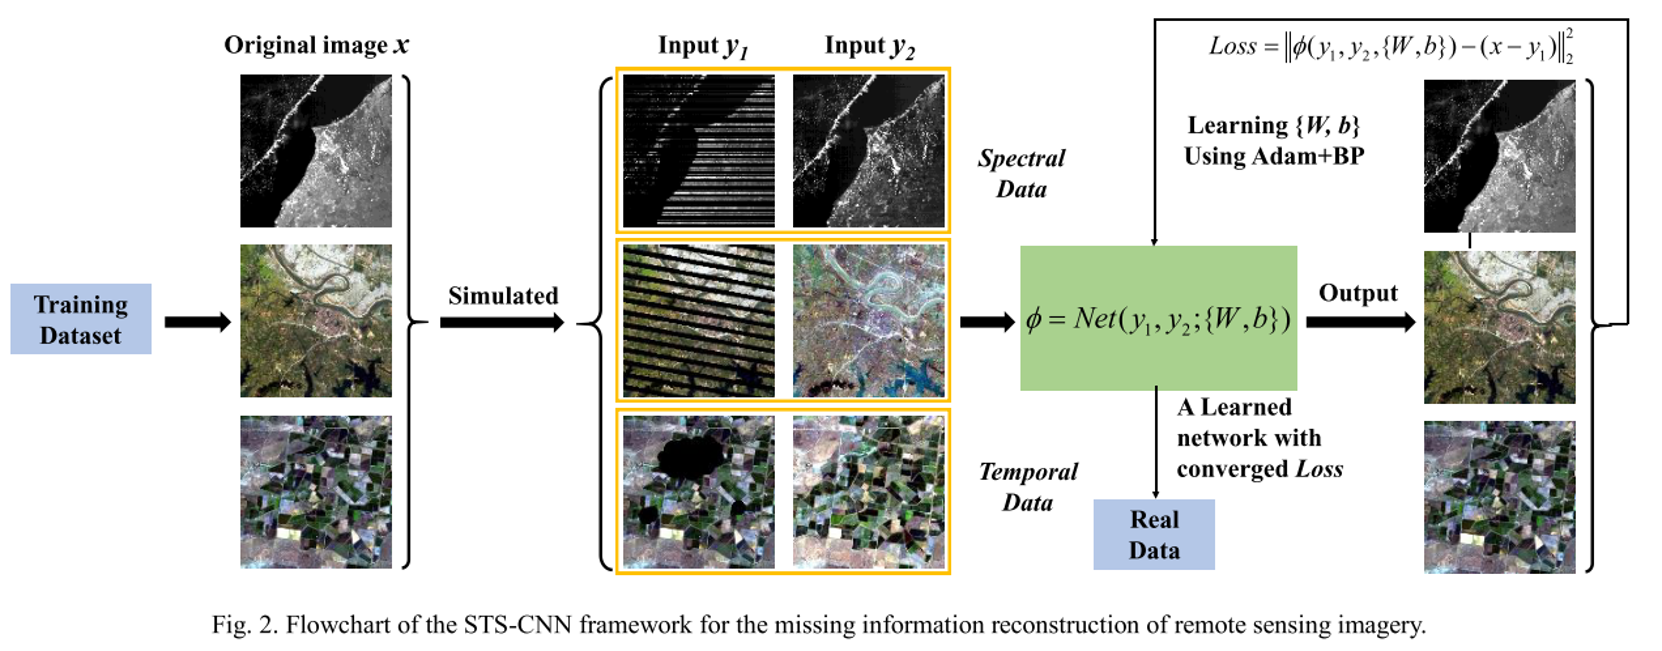
\includegraphics[width=1\textwidth]{figures/sts-cnn_framework.png}
	\caption{For example of Unified Spatial-Temporal-Spectral Deep Convolutional Neural Network, Qiang et al., they use only one image as referenced image and \textit{temporal} just means \textit{at different times}, not use periodicity attribute of weather.}
\end{figure}

\section {Dataset}
In this chapter, Tri An reservoir is chosen for experimetns, because it has enough large area for visualization, segmentation and calculation. Each tile from satellite imagery can only focus on part of the Earth, and Tri An reservoirs' water body belongs to one tile, so that it is not necessary to concatenate many tiles.

\begin{figure}[h!]
	\centering
	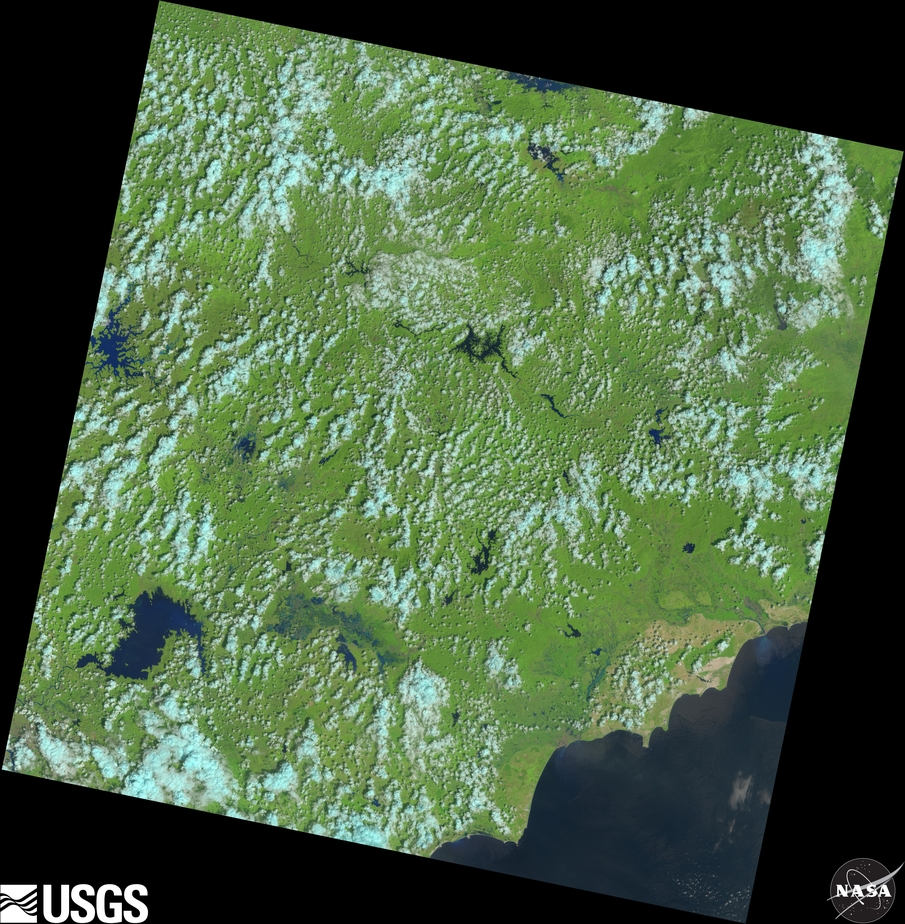
\includegraphics[width=0.6\textwidth]{figures/l8tile.png}
	\caption{Tri An Reservoir belongs to a tile of Landsat 8 data file. Date taken: January 10, 2013}
\end{figure}	


We use Landsat 8 data for optical satellite. For radar satellite, Sentinel-1 images are chosen. Those data can be freely acquired from the Internet.

\subparagraph{Requiring time period} \textbf{Landsat 8} data files are collected in period November 2013 - May 2018. SAR Imagery from \textbf{Sentinel-1} are from April 2014 - May 2018.

\section{Model}

In this method, we will refer a neural network of STS-CNN\cite{Zhang2018} to re-implement a neural network to our data. 

This algorithm has 3 inputs: (1) A missing image, (2) a referenced image and a missing image (1) with damaged regions filled by corresponding region in referenced image. The output is a recovered image. Note that, we have three images as input, and the third aims to tell a neural network easier to determine which are missing regions on the images. The referenced image will be also taken from Landsat 8, on cloudy-free day. For equal comparison to original method, we will use example of masks that provided with this paper, can be found at: \href{https://github.com/WHUQZhang/STS-CNN/}{https://github.com/WHUQZhang/STS-CNN/}.

The optimizer function is $Adam$ and the learning rate of whole network is $1e-4$. See at Figure \ref{fig:modifiedModel}.

\begin{figure}[h!tb]
	\clearpage{}
	\centering
	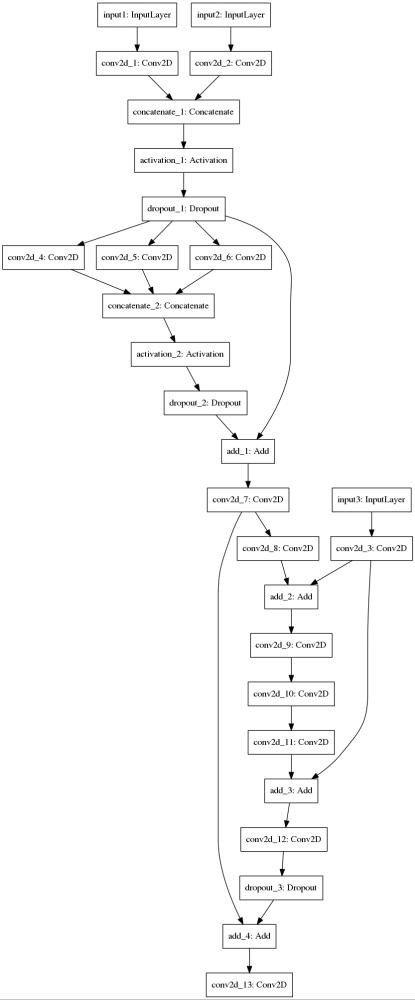
\includegraphics[width=0.6\textwidth]{figures/modifiedModel.png}
	\caption{Modified model, with 3 of inputs. \textit{Input 1}: Missing image. \textit{Input 2}: Referenced image. \textit{Input 3}: Referenced with simulated-missing regions like \textit{Input 1}}
	\label{fig:modifiedModel}
\end{figure}	

For comparison, we will use cloud-free image and add on it two type mask to feed into network. The first type is a simple shape mask from original method. The second is get from QA Bands of one cloud day, which is acquired by Landsat 8. In order to get cloud cover, F-mask program (Python, \href{http://pythonfmask.org}{http://pythonfmask.org}) is used to get cloud mask from QA Bands. The table shows difference between original method and my re-implemented method. For more visualization, take a look at figure \textit{4.1} in \textbf{Experiment}. For measuring between methods, in this chapter, we use Peak signal-to-noise ratio.

\subparagraph{Peak signal-to-noise ratio} \textit{Wikipedia} It often abbreviated $PSNR$, is an engineering term for the ratio between the maximum possible power of a signal and the power of corrupting noise that affects the fidelity of its representation. Because many signals have a very wide dynamic range, $PSNR$ is usually expressed in terms of the logarithmic decibel scale. 

\begin{equation}
\centering
PSNR \textrm{ = } 20 * log_{10}(MAX_I) - 10 * log_{10}(MSE)
\end{equation}

where $MAX_I$ is the maximum possible value of image $I$, depending on its depth. For example, if the pixels are represented using 8 bits per sample ($8-bit$ image), this is 255. More generally, when samples are represented using linear PCM with $B$ bits per sample, $MAX_I$ is $2^B$ $-$ $1$. \textit{Mean square error}, $MSE$, between the original image $I$ with predicted image $K$, with the same of size ($m, n$) will be calculated as following:

\begin{equation}
\centering
MSE \textrm{ = } \frac{1}{mn} \sum_{i \textrm{ = } 1}^{m} \sum_{j \textrm{ = } 1}^{n} [I_{i,j} - K_{i,j}]^2
\end{equation}

\vspace{0.3cm}
Table of comparison:

\begin{table}[h!]
	\centering
	\begin{tabular}{|c|c|c|c|}
		\hline
		& STS-CNN & \begin{tabular}[c]{@{}c@{}}Modified model \\ (0..1)\end{tabular} & \begin{tabular}[c]{@{}c@{}}Modified model \\ (0..255)\end{tabular} \\ \hline
		Simple cloud         & 19.9098 & \textbf{27.00188}                                                & 26.7391                                                            \\ \hline
		Simple multi-cloud   & 15.6941 & \textbf{23.8445}                                                 & 23.80995                                                           \\ \hline
		Real (complex) cloud & 12.8381 & \textbf{19.70776}                                                & 19.5976                                                            \\ \hline
	\end{tabular}
	\caption{Comparison between proposed model to modified model. Pixel value are scale to $(0..1)$ and $(0..255)$ (original has pixel range from $0..65535$). All are calculated by $PSNR$. Higher is better}
\end{table}

\section{Optimization}

As periodicity of weather is being used for higher accuracy in recovering water body, we use two methods below on our dataset: (1) \textbf{Using Time-Distributed Layer from Keras}; (2) \textbf{Recurrent-CNN}, which uses a kind of Recurrent Neural Network, Long-Short Term Memory. A common thing between between two approaches is applying a temporal slice of images into neural network, and the purpose of those sub-networks is predicting the next images to be referenced image. 

\subsection{Using Time-Distributed Layer from Keras}

Keras framework also provides Time-Distributed layers, which applies for every temporal slice of an input. Because of limitation of hardware memory, we feed into it five consecutive images acquired from Landsat 8. For referenced image, we try with 2 type: first is Landsat 8 and the second is Sentinel-1. Because only water body is focused, so we've classified water body on Sentinel-1 data, and resize it to the same of Landsat 8 (Sentinel-1 has 10 meters of resolution). Model specification contains 2 part: \textit{part 1}  (at Fig. \ref{fig:timemodelPart1}) is about using Time-Distributed to get predicted image as reference, \textit{part 2} (at Fig. \ref{fig:timemodelPart2}) is quite similar to existing method for reconstruction.

\begin{figure}[h!]
	\centering
	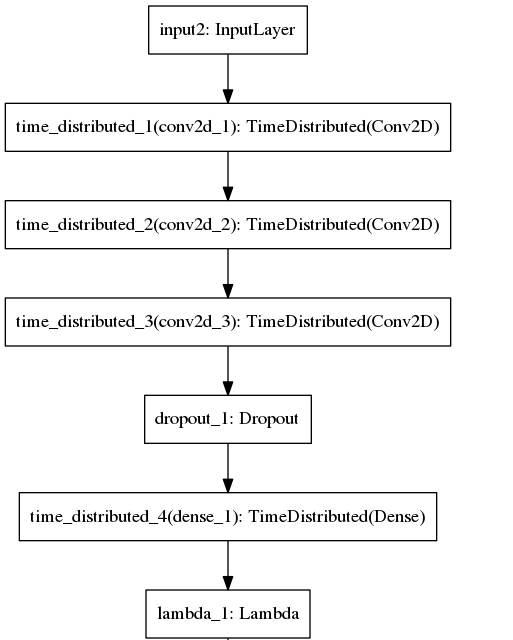
\includegraphics[width=0.5\textwidth]{figures/timemodelPart1.png}
	\caption{Applying Time-Distributed in Neural Network. Lambda is a function to get 1-time next predicted image from time-series images to be reference image.}
	\label{fig:timemodelPart1}
\end{figure}

\begin{figure}[h!]
	\centering
	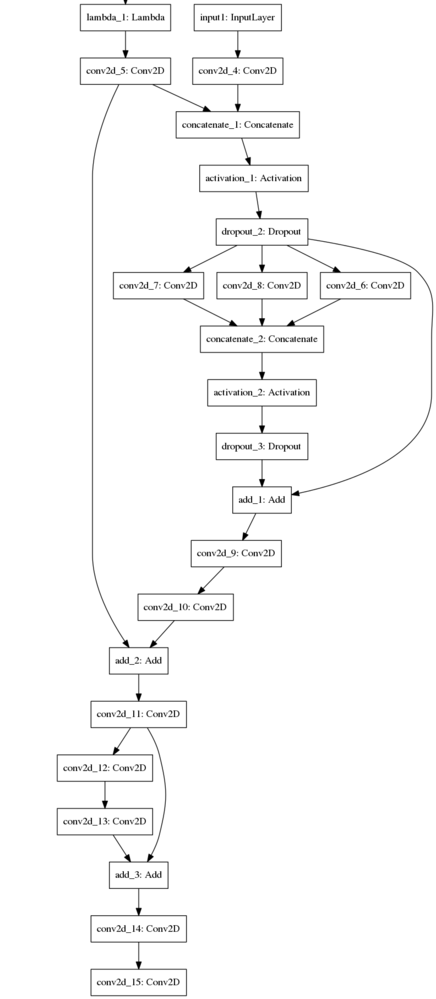
\includegraphics[width=0.7\textwidth]{figures/timemodelPart2.png}
	\caption{Using predicted image as reference image, with part in order to reconstruct missing regions. Note that there is not input \textit{referenced image with missing data}}
	\label{fig:timemodelPart2}
\end{figure}

\subsection{Recurrent-CNN implementation}

The idea behind Recurrent Neural Networks (RNNs) is to make use of sequential information. So that, this approach aims to use Long Short Term Memory networks – usually just called “LSTMs” – are a special kind of RNN, capable of learning long-term dependencies, to make prediction of next image, based on five consecutive images, and use the next image as referenced image for reconstruction. For the predictive part, see \ref{fig:modelConv2DLSTM_1}. The main is similar to  \ref{fig:timemodelPart2}

\begin{figure}[h!]
	\centering
	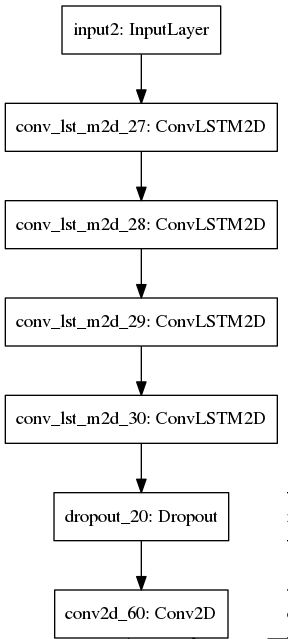
\includegraphics[width=0.5\textwidth]{figures/modelConv2DLSTM_1.png}
	\caption{LSTM (as Conv2DLSTM Layer) aims to predict the next image to be used as referenced image}
	\label{fig:modelConv2DLSTM_1}
\end{figure}

\subsection{Comparison}

This is a comparison between above methods. Input 1 is damaged image,  input 2 is a time-series data (5 images).

\begin{table}[h!]
	\centering
	\begin{tabular}{|c|c|c|}
		\hline
		& \begin{tabular}[c]{@{}c@{}}Time-Distributed\\ Layers\end{tabular} & LSTM-Conv2D \\ \hline
		Simple cloud         & \textbf{30.5584}                                                  & 23.4441     \\ \hline
		Simple multi-cloud   & \textbf{29.9230}                                                  & 24.0554     \\ \hline
		Real (complex) cloud & \textbf{30.4467}                                                  & 26.4210     \\ \hline
	\end{tabular}
	\caption{Comparison when applying time-series images for predicting next image as reference.}
\end{table}

\section{Experiments}

\subsection{One reference image - Comparison with original method}

In this section, we take an example from testing data. Band 3, 4, 5 \textit{(Red, Green, Near IR from Landsat 8)} were chosen for making RGB image. For image within range $0..1$, after reconstructed, we multiply for each pixel by 255.
\begin{figure}[h!]
	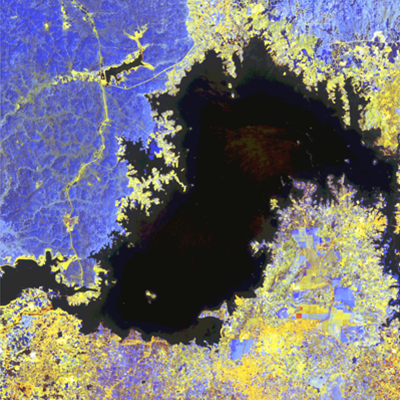
\includegraphics[width=0.7\linewidth]{figures/groud_truth.png}
	\centering
	\caption{Ground Truth}
\end{figure}

\subsubsection{Easiest case: Simple cloud shape}

\begin{figure}[h!]
	\centering
	\subfloat[]{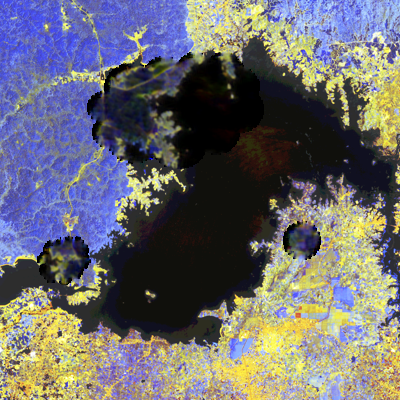
\includegraphics[width=0.32\linewidth]{figures/sts_sample_cloud.png}}
	\subfloat[]{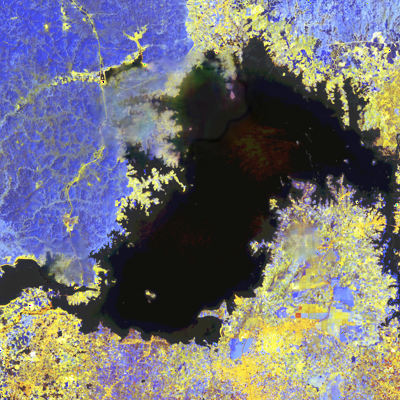
\includegraphics[width=0.32\linewidth]{figures/1_simple.png}}
	\subfloat[]{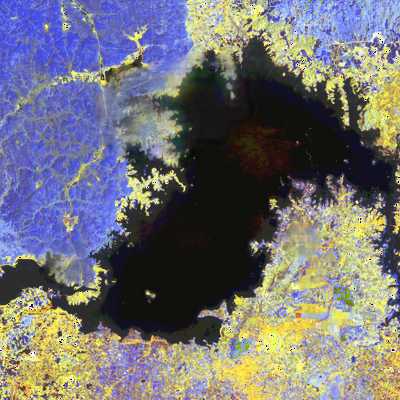
\includegraphics[width=0.32\linewidth]{figures/255_simple.png}} 

	\centering
	\caption{
		\textbf{(a)} STS-CNN.
		\textbf{(b)} Modified Model, range $0..1$.
		\textbf{(c)} Modified Model, range $0..255$}
\end{figure}


\subsubsection{Average case: Multi-simple cloud shape}

\begin{figure}[h!]
	\centering
	\subfloat[]{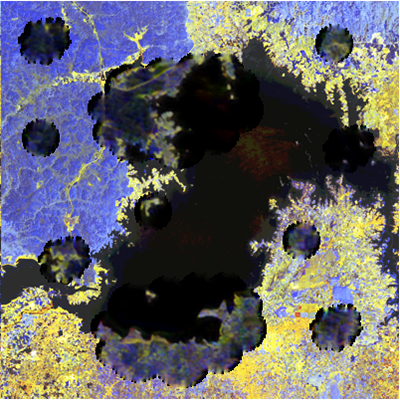
\includegraphics[width=0.32\linewidth]{figures/sts_sample_multicloud.png}}
	\subfloat[]{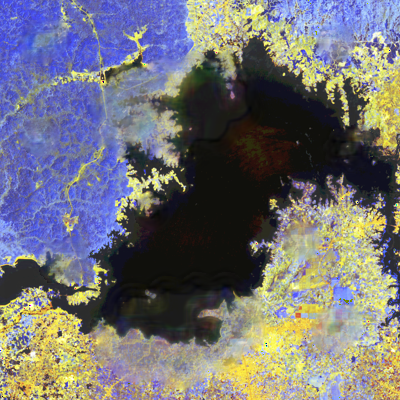
\includegraphics[width=0.32\linewidth]{figures/1_multiFake.png}}
	\subfloat[]{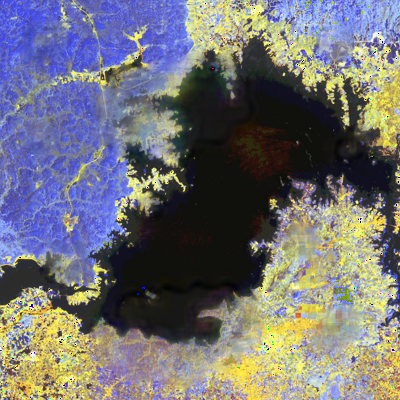
\includegraphics[width=0.32\linewidth]{figures/255_multi_fake.png}} 

	\centering
	\caption{
		\textbf{(a)} STS-CNN.
		\textbf{(b)} Modified Model, range $0..1$.
		\textbf{(c)} Modified Model, range $0..255$}
\end{figure}

\subsubsection{Hardest case: Real cloud}

\begin{figure}[h!]
	\centering
	\subfloat[]{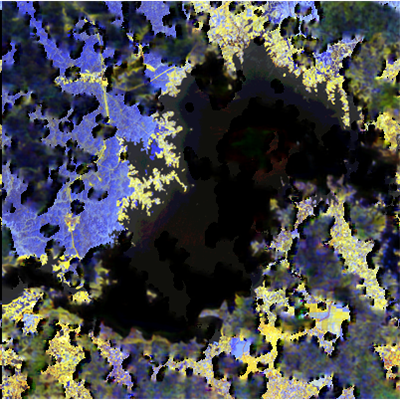
\includegraphics[width=0.32\linewidth]{figures/sts_real_cloud.png}}
	\subfloat[]{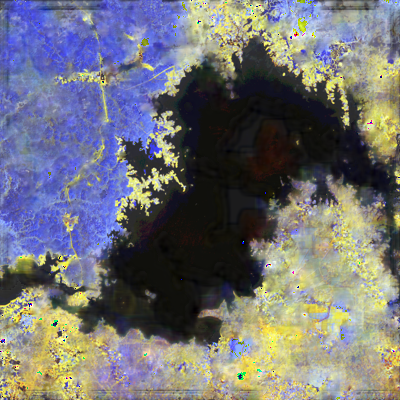
\includegraphics[width=0.32\linewidth]{figures/1_complex.png}}
	\subfloat[]{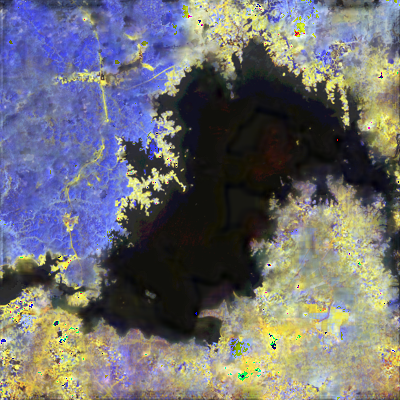
\includegraphics[width=0.32\linewidth]{figures/255_complex.png}} 
	
	\centering
	\caption{
		\textbf{(a)} STS-CNN.
		\textbf{(b)} Modified Model, range $0..1$.
		\textbf{(c)} Modified Model, range $0..255$}
\end{figure}


\subsection{Trying to recover water body}
Model has been trained in \textbf{4.1} to take experiments on recovering water body from reconstructed images in cloud days. In order to recover water body, images are collected from Landsat 8 will be crop to be size of $1200 x 1600$ pixels, equals $3 x 4$ tiles, each tiles has size of $400 x 400$ pixels.  

For segmentation, NDWI-index is used to mask out water body. For comparison to ground truth, the most nearest SAR-image collected from Sentinel-1 will be used. 

All Landsat 8 images has been calculated by NDWI formula:

\begin{equation}
NDWI = \frac{Green - Near IR}{Green + Near IR}
\end{equation}

and the display images only contain pixel that having NDWI-index above 0 (which are water or cloud pixel). For Sentinel-1 images, VH-band is used. The pixel belongs to water have value less than -22.

\subparagraph{Explanation for figures} Note that, \textbf{(a)} is covered by cloud, \textbf{(b)} is recovered and \textbf{(c)} is collected from Sentinel-1. 

\begin{figure}[h!]
	\centering
	\subfloat[60.6114 $km^2$]{
		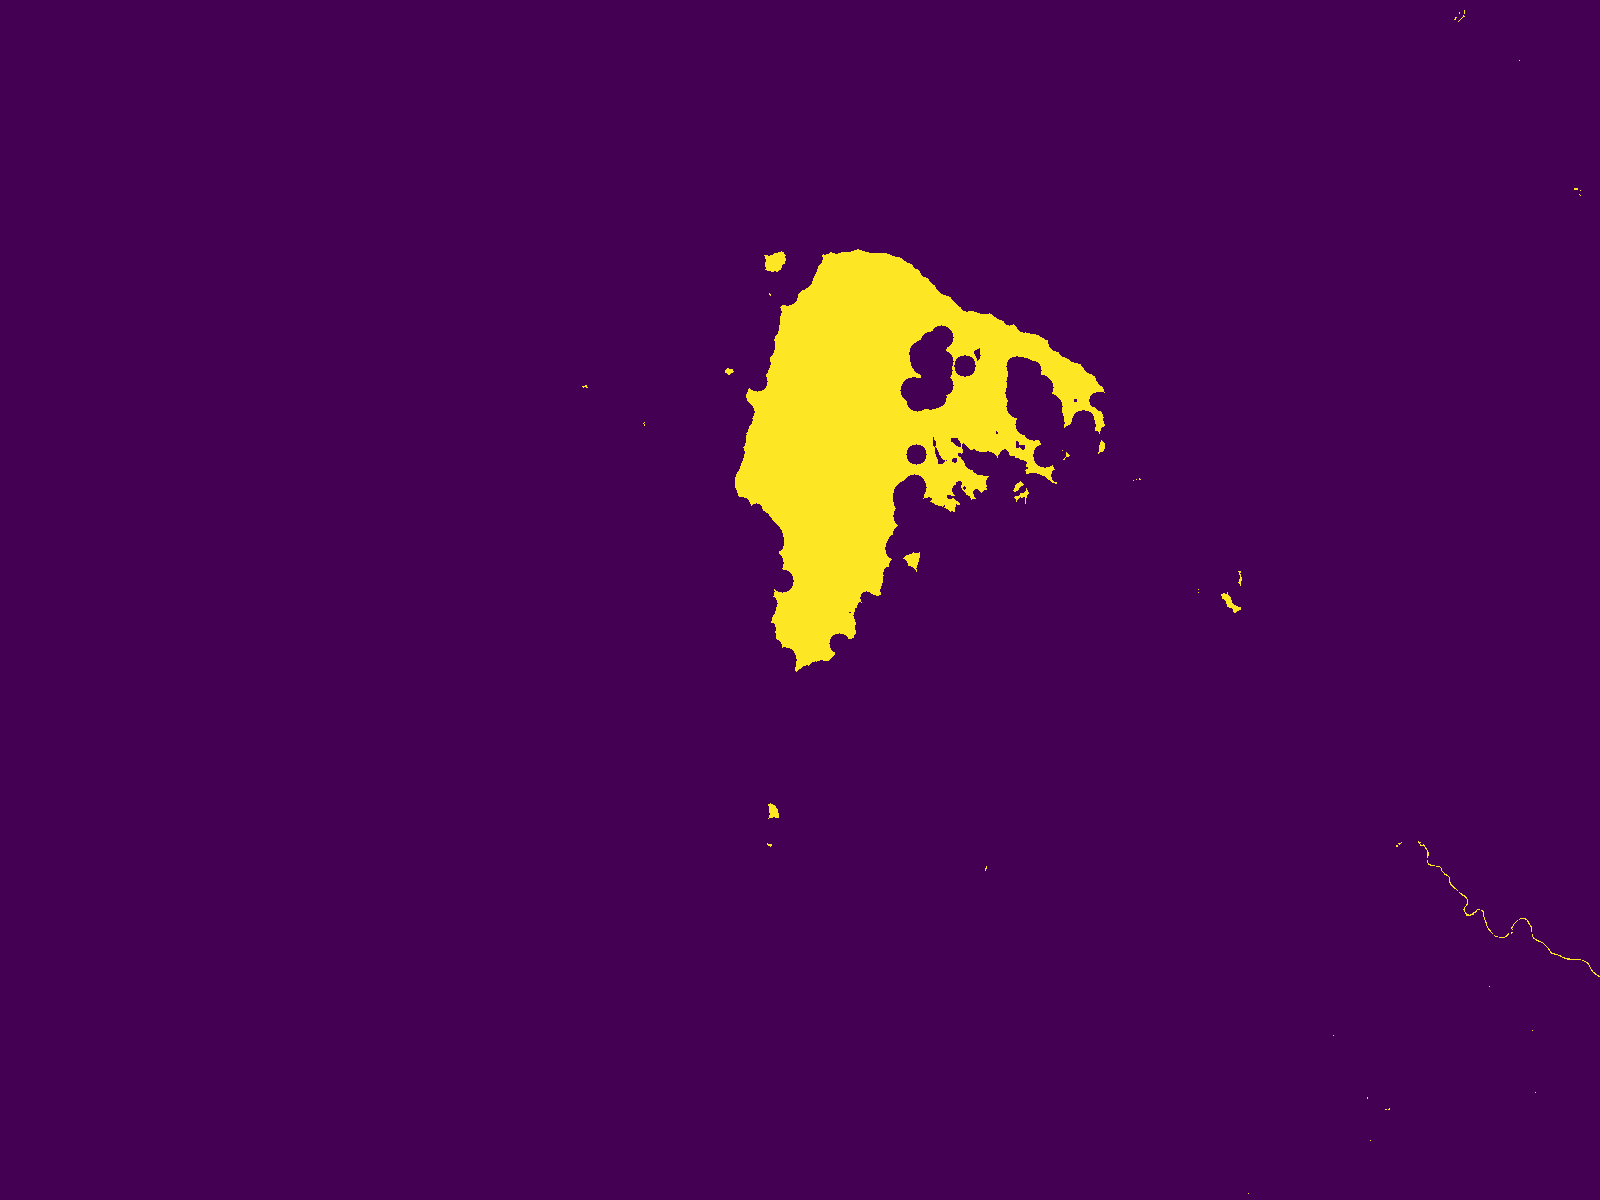
\includegraphics[width=0.32\linewidth]{figures/raw20160104_60_6114.png}
	}
	\subfloat[242.0488 $km^2$]{
		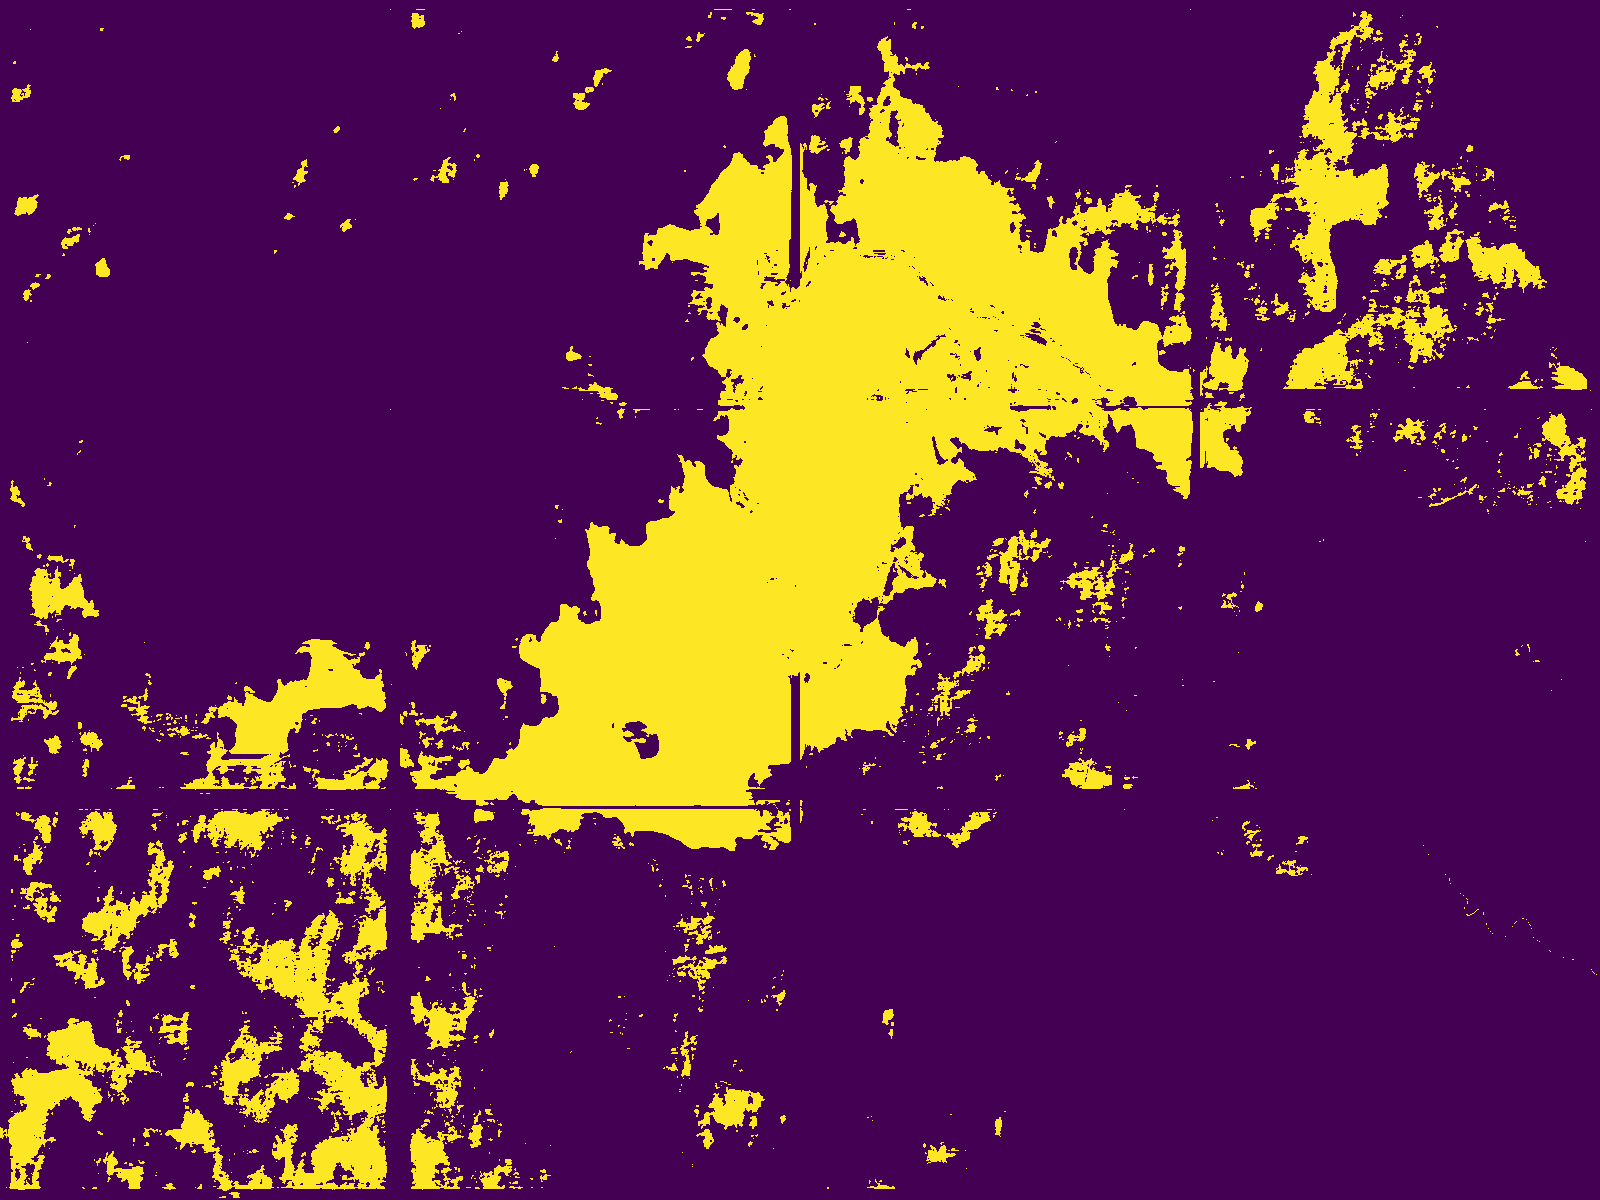
\includegraphics[width=0.32\linewidth]{figures/r20160104_242_0488.png}
	}
	\subfloat[269.2041 $km^2$]{
		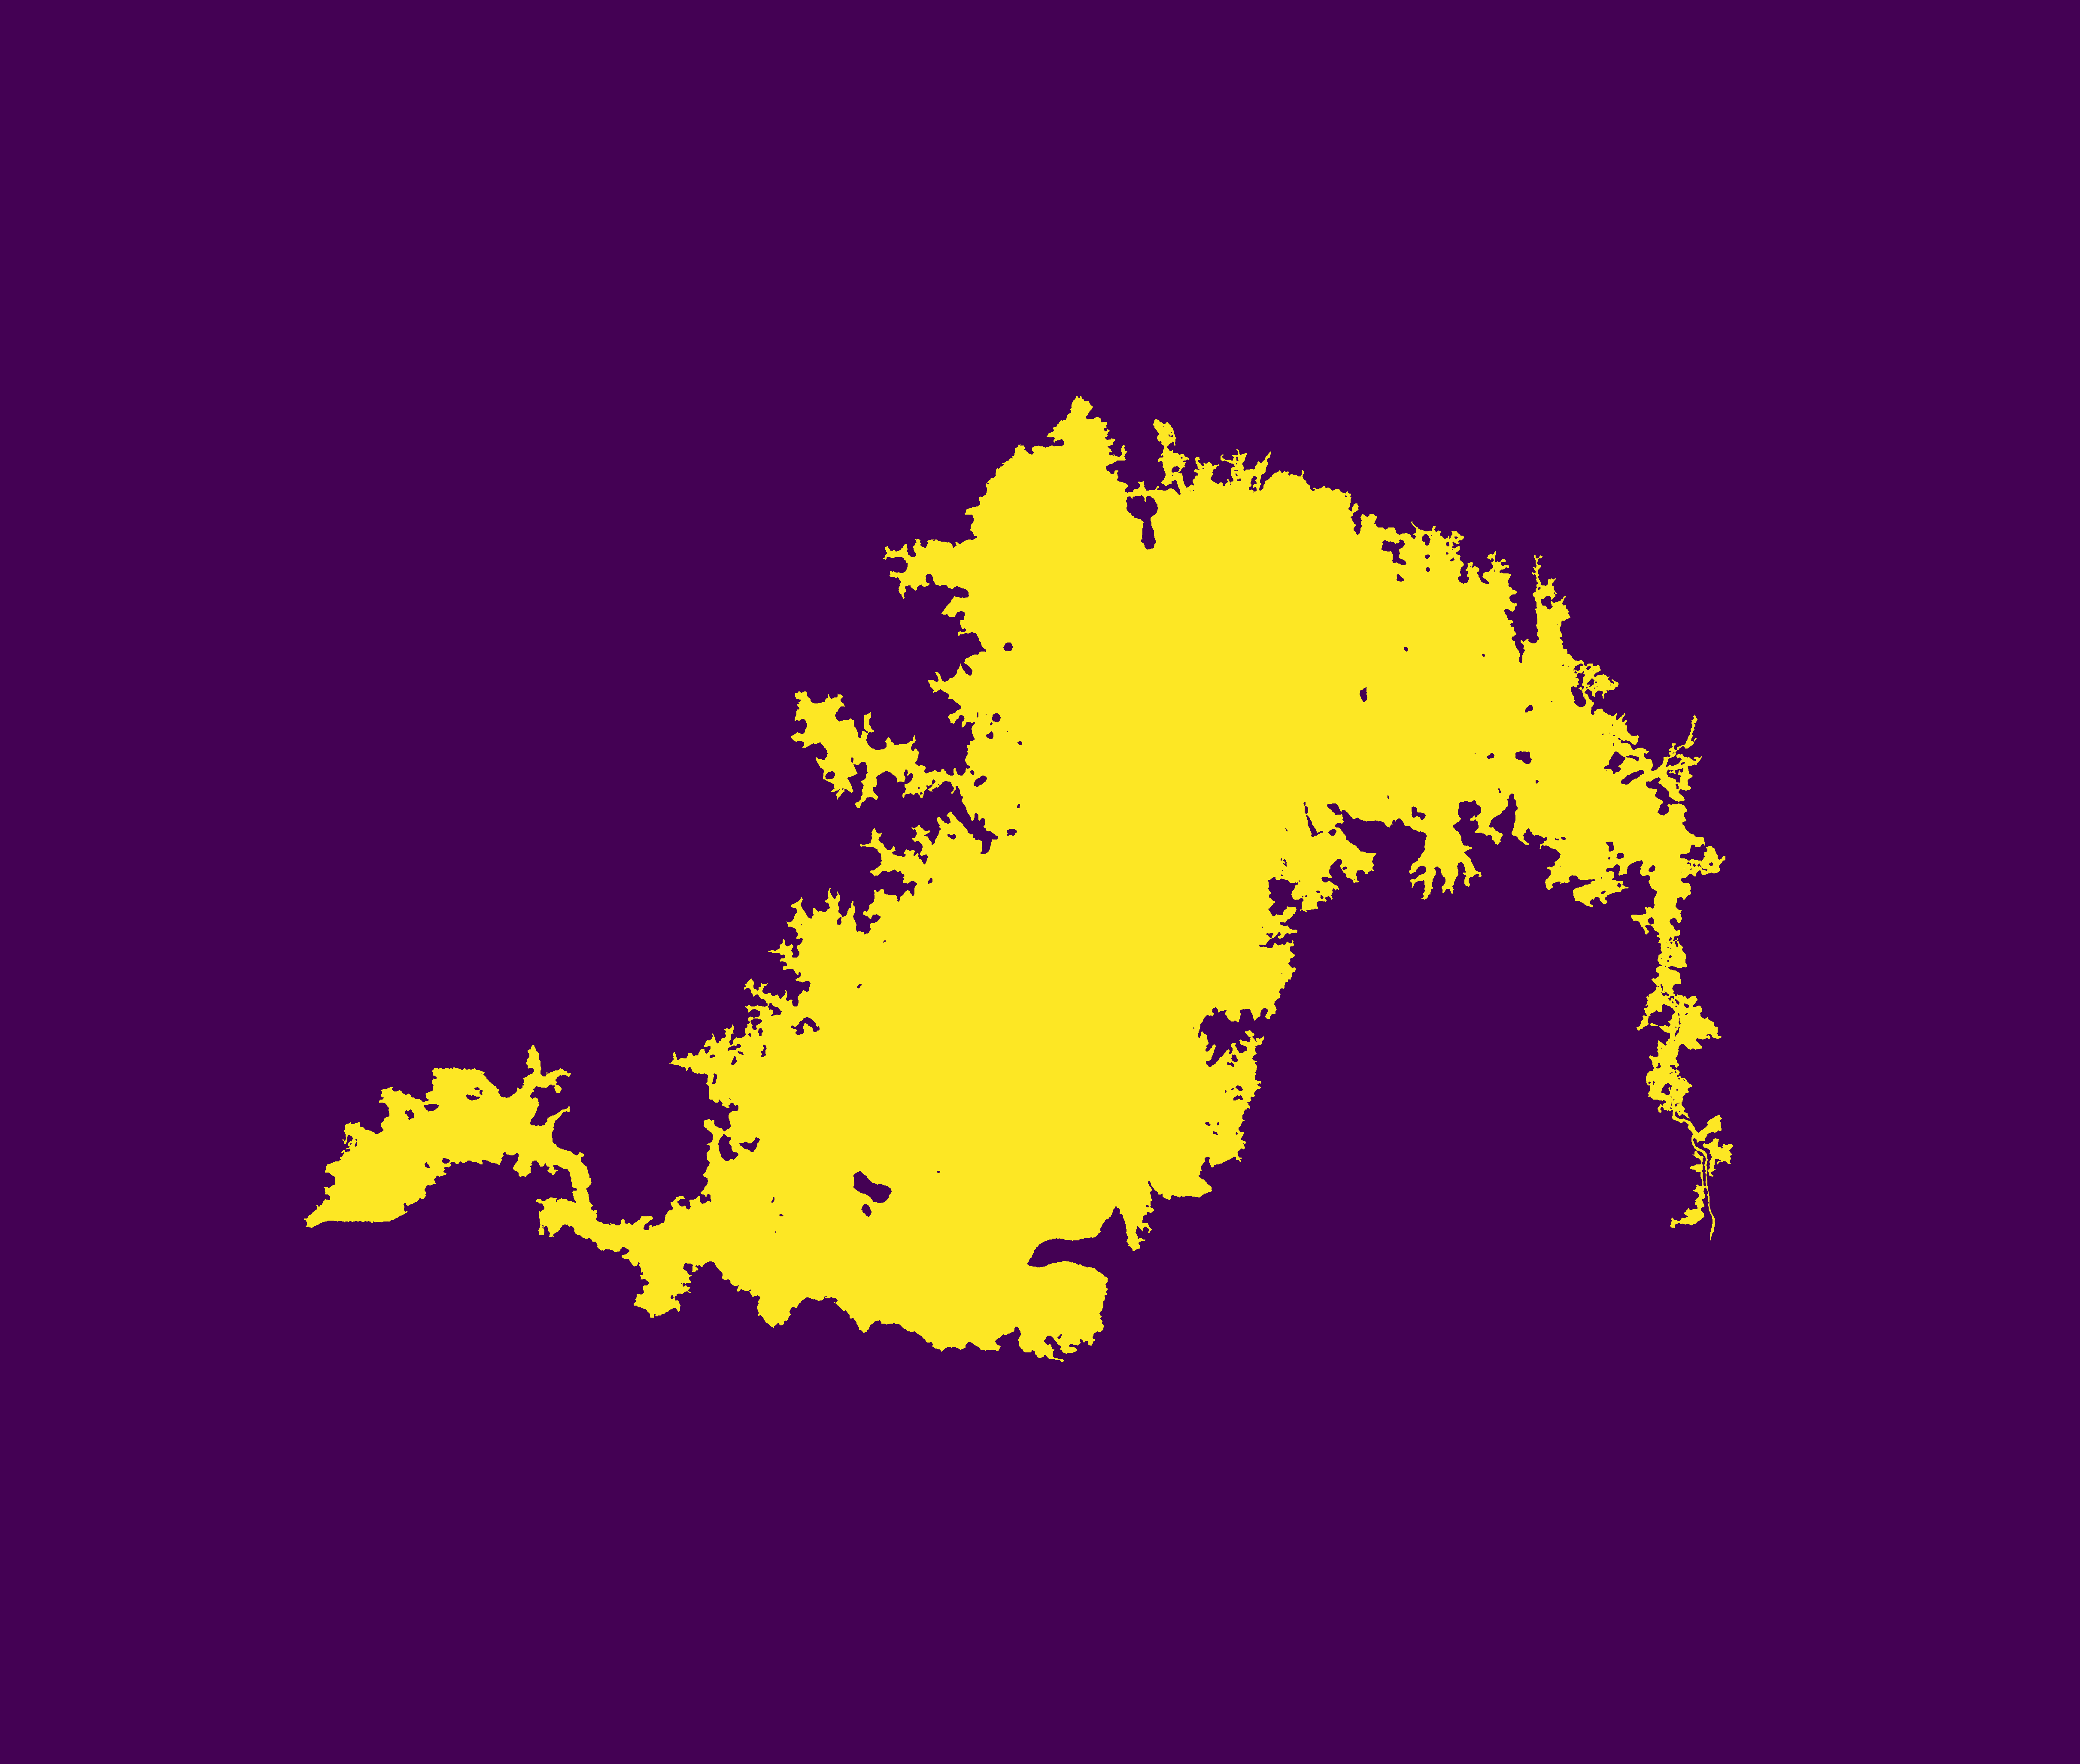
\includegraphics[width=0.32\linewidth]{figures/20160112_269_2041.png}
	} 
	
	\centering
	\caption{
		\textbf{(a, b)} Landsat 8, Jan 4th 2016.
		\textbf{(c)} Sentinel-1, Jan 12th 2016.}
\end{figure}


\begin{figure}[h!]
	\centering
	\subfloat[51.8346 $km^2$]{
		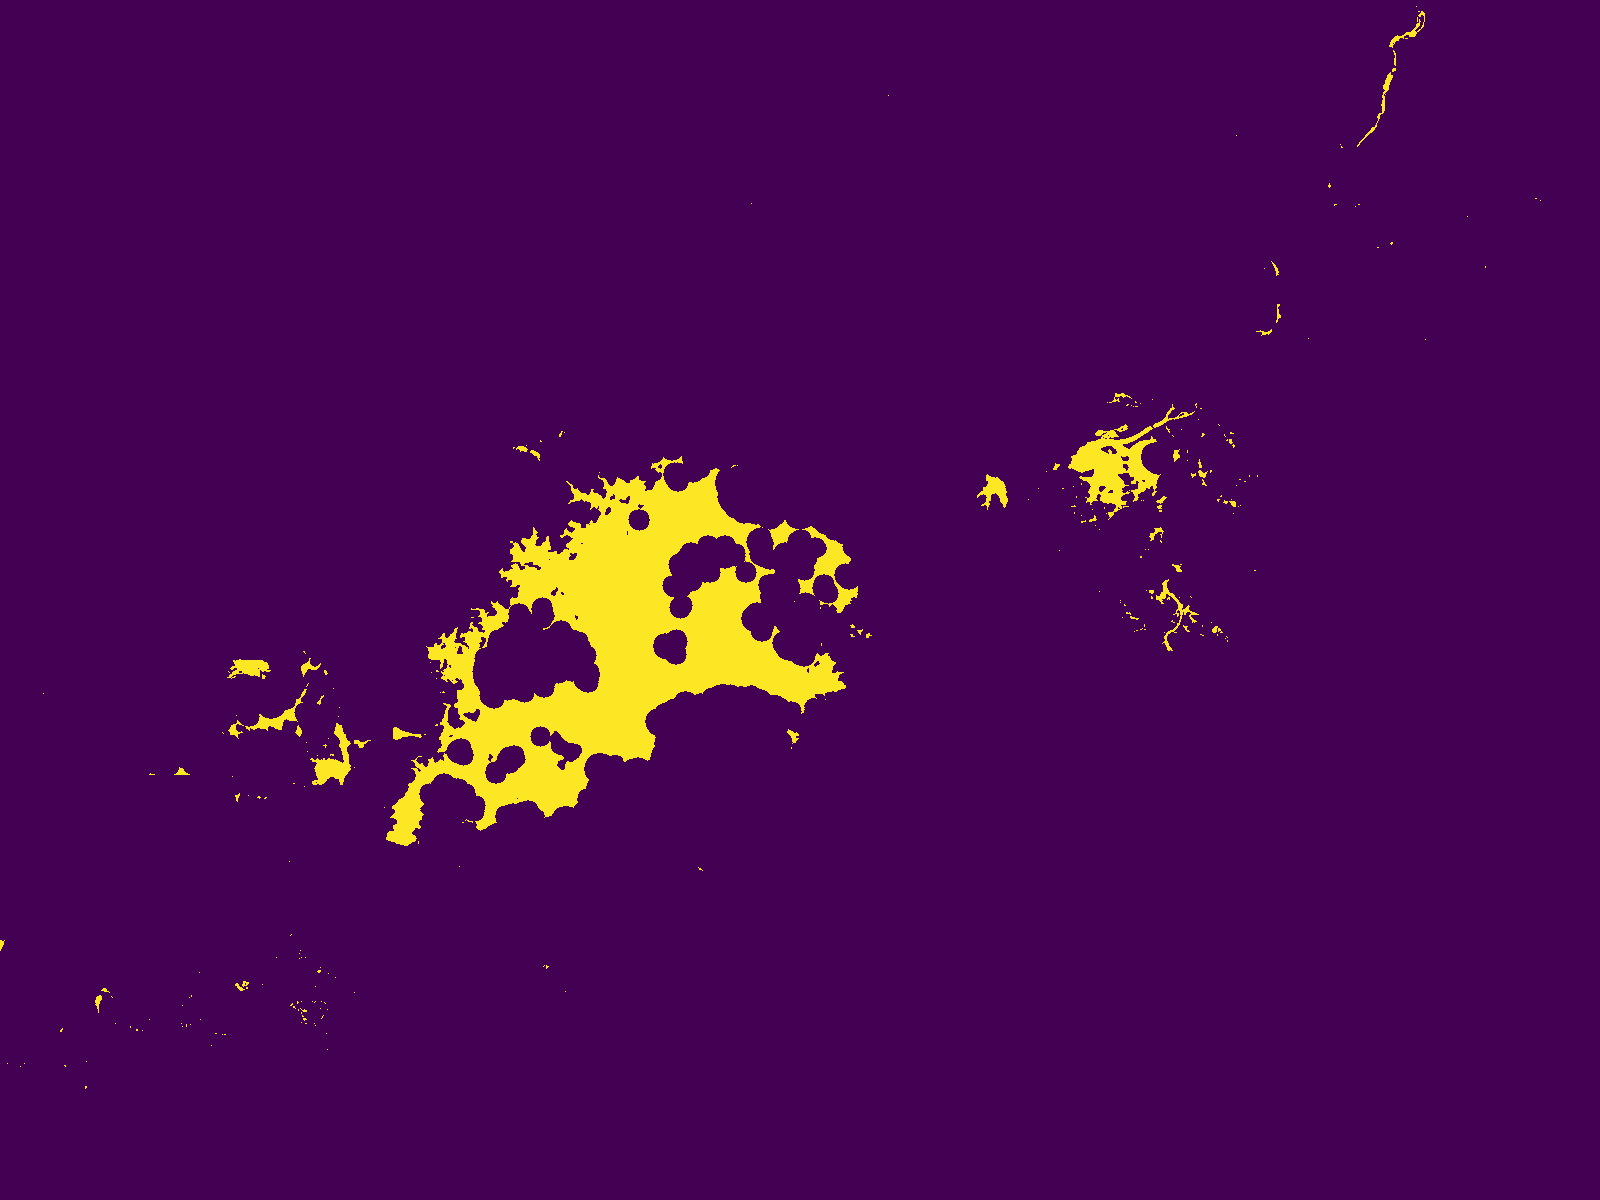
\includegraphics[width=0.32\linewidth]{figures/raw20160815_51_8346.png}
	}
	\subfloat[193.9509 $km^2$]{
		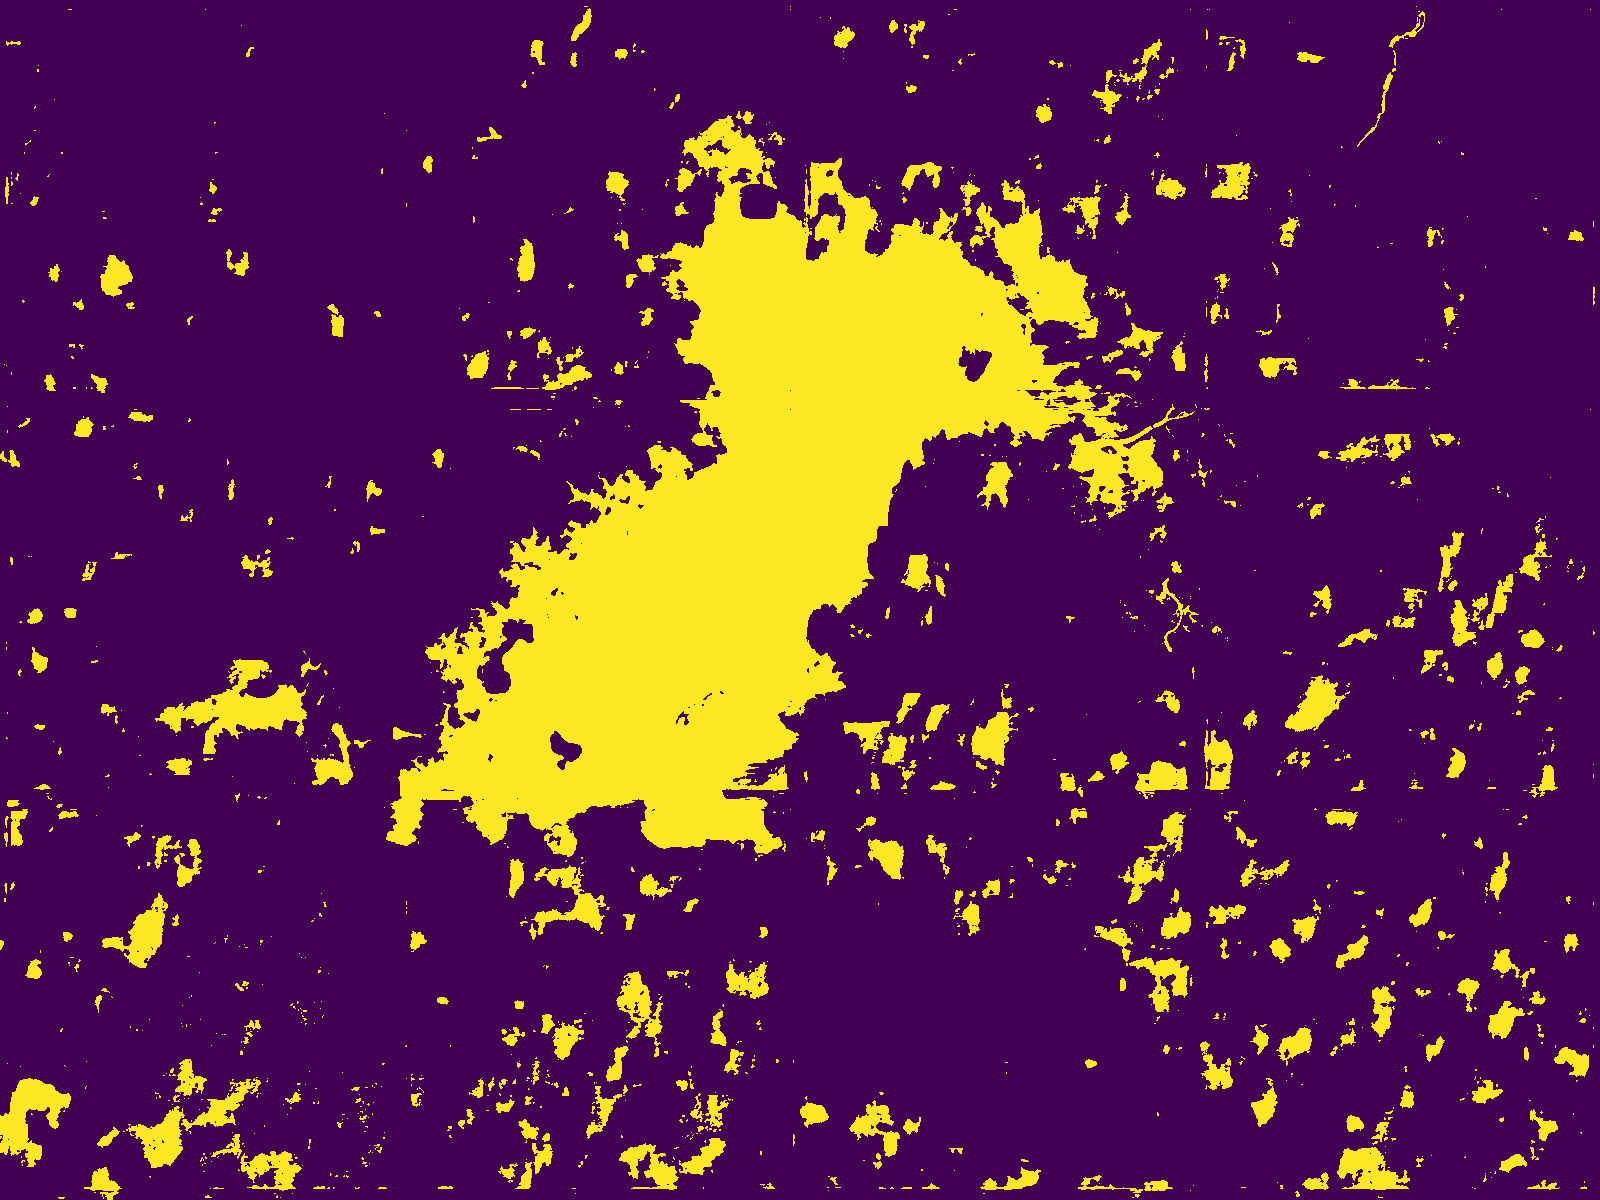
\includegraphics[width=0.32\linewidth]{figures/r20160815_193_9509.png}
	}
	\subfloat[201.6019 $km^2$]{
		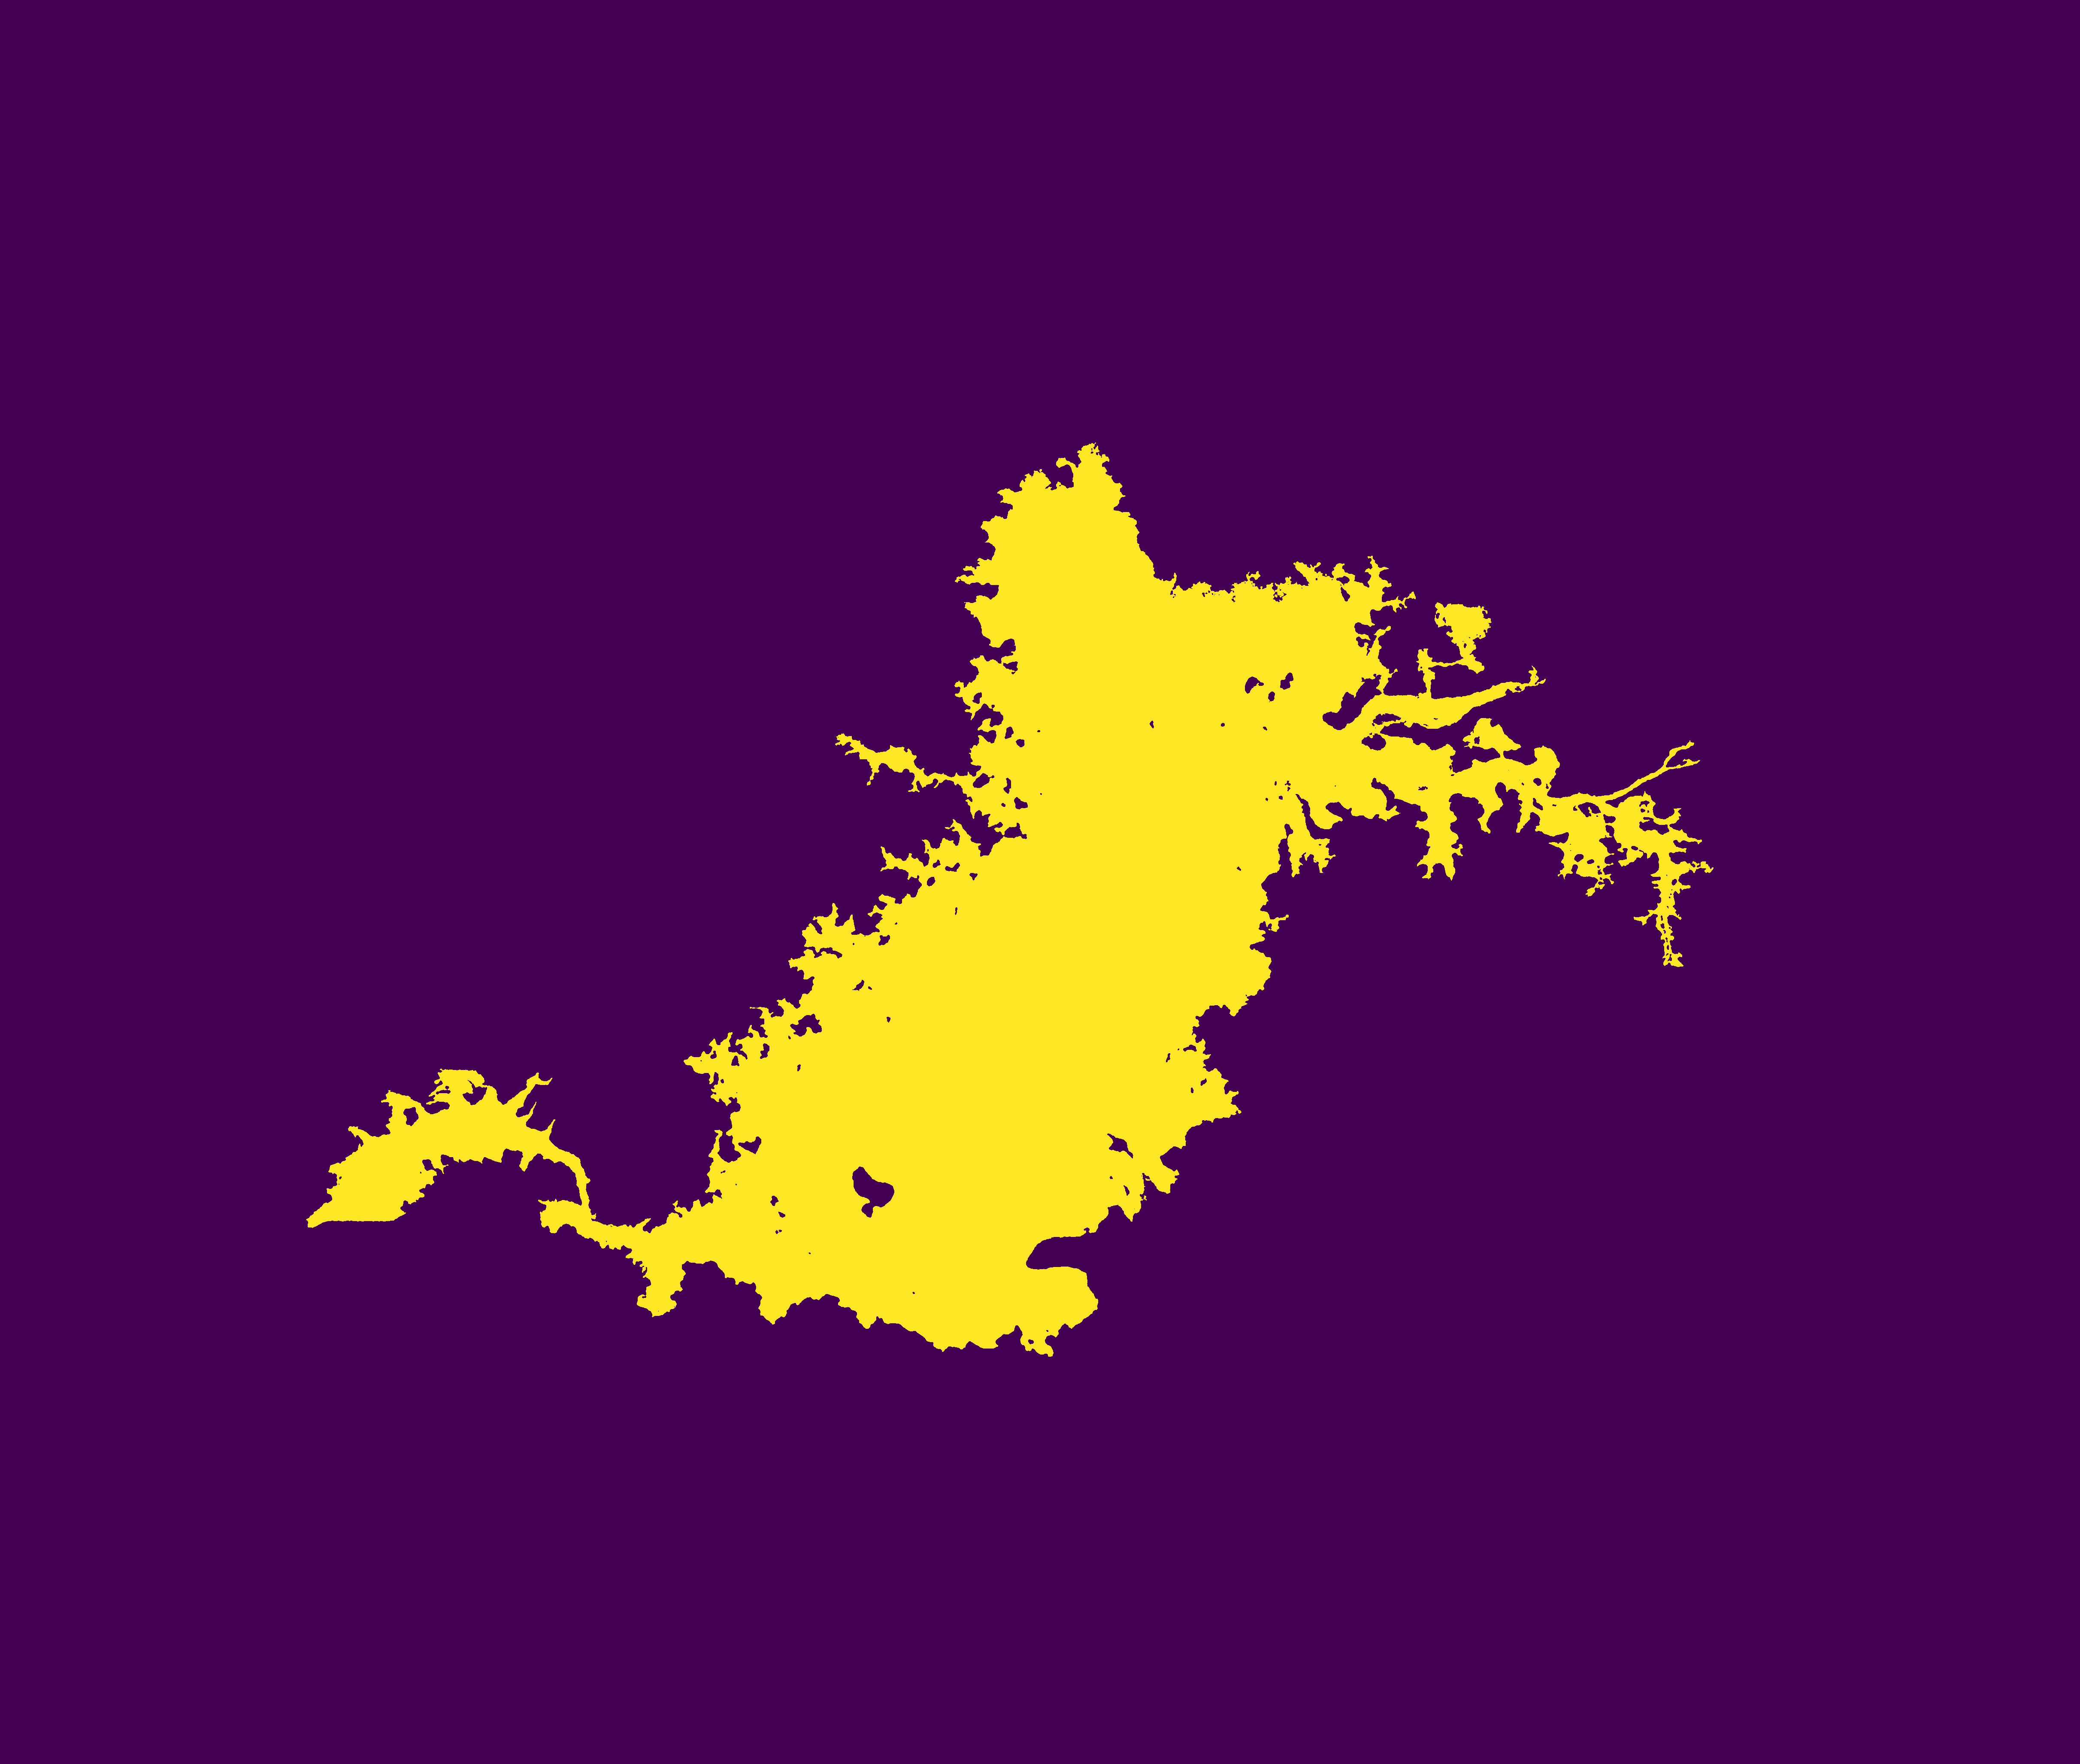
\includegraphics[width=0.32\linewidth]{figures/20160815_201_6019.png}
	} 
	
	\centering
	\caption{
		\textbf{(a, b)} Landsat 8, Aug 15th 2016.
		\textbf{(c)} Sentinel-1, Aug 15th 2016.}
	\end{figure}


\begin{figure}[h!]
\centering
\subfloat[31.2336 $km^2$]{
	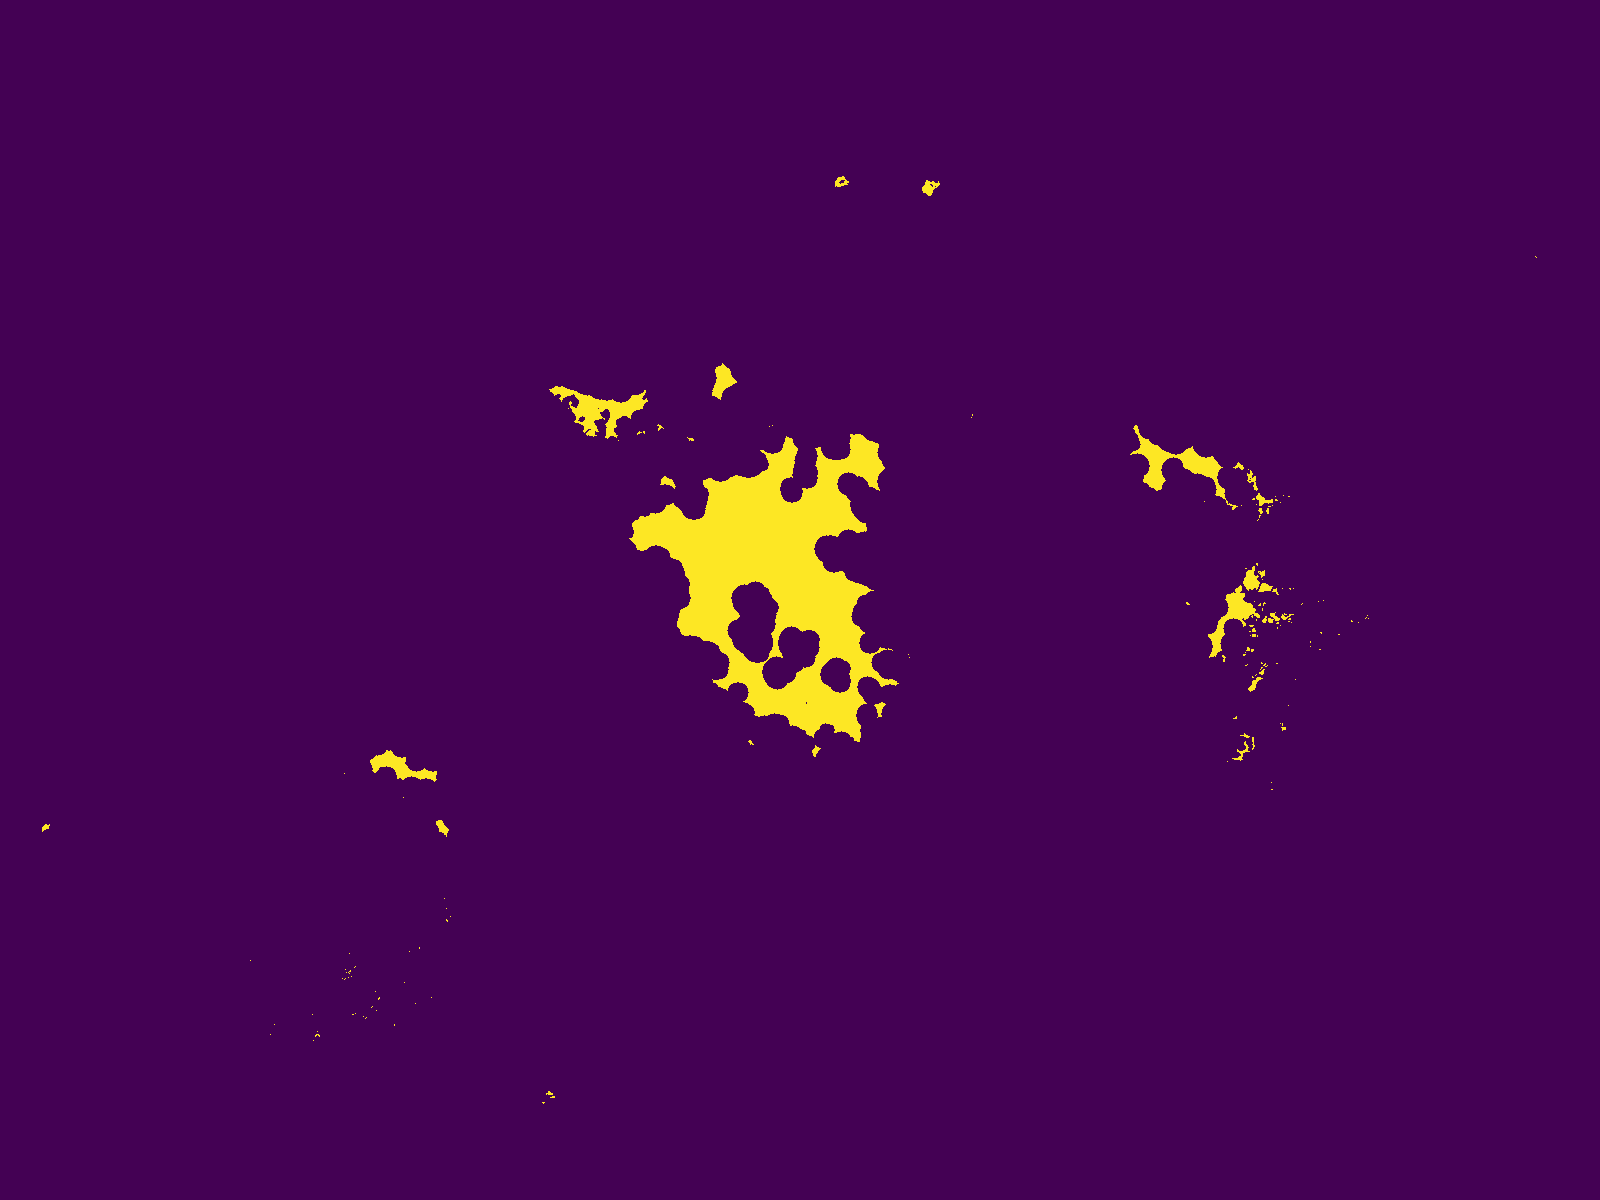
\includegraphics[width=0.32\linewidth]{figures/raw20170802_31_2336.png}
}
\subfloat[185.7141 $km^2$]{
	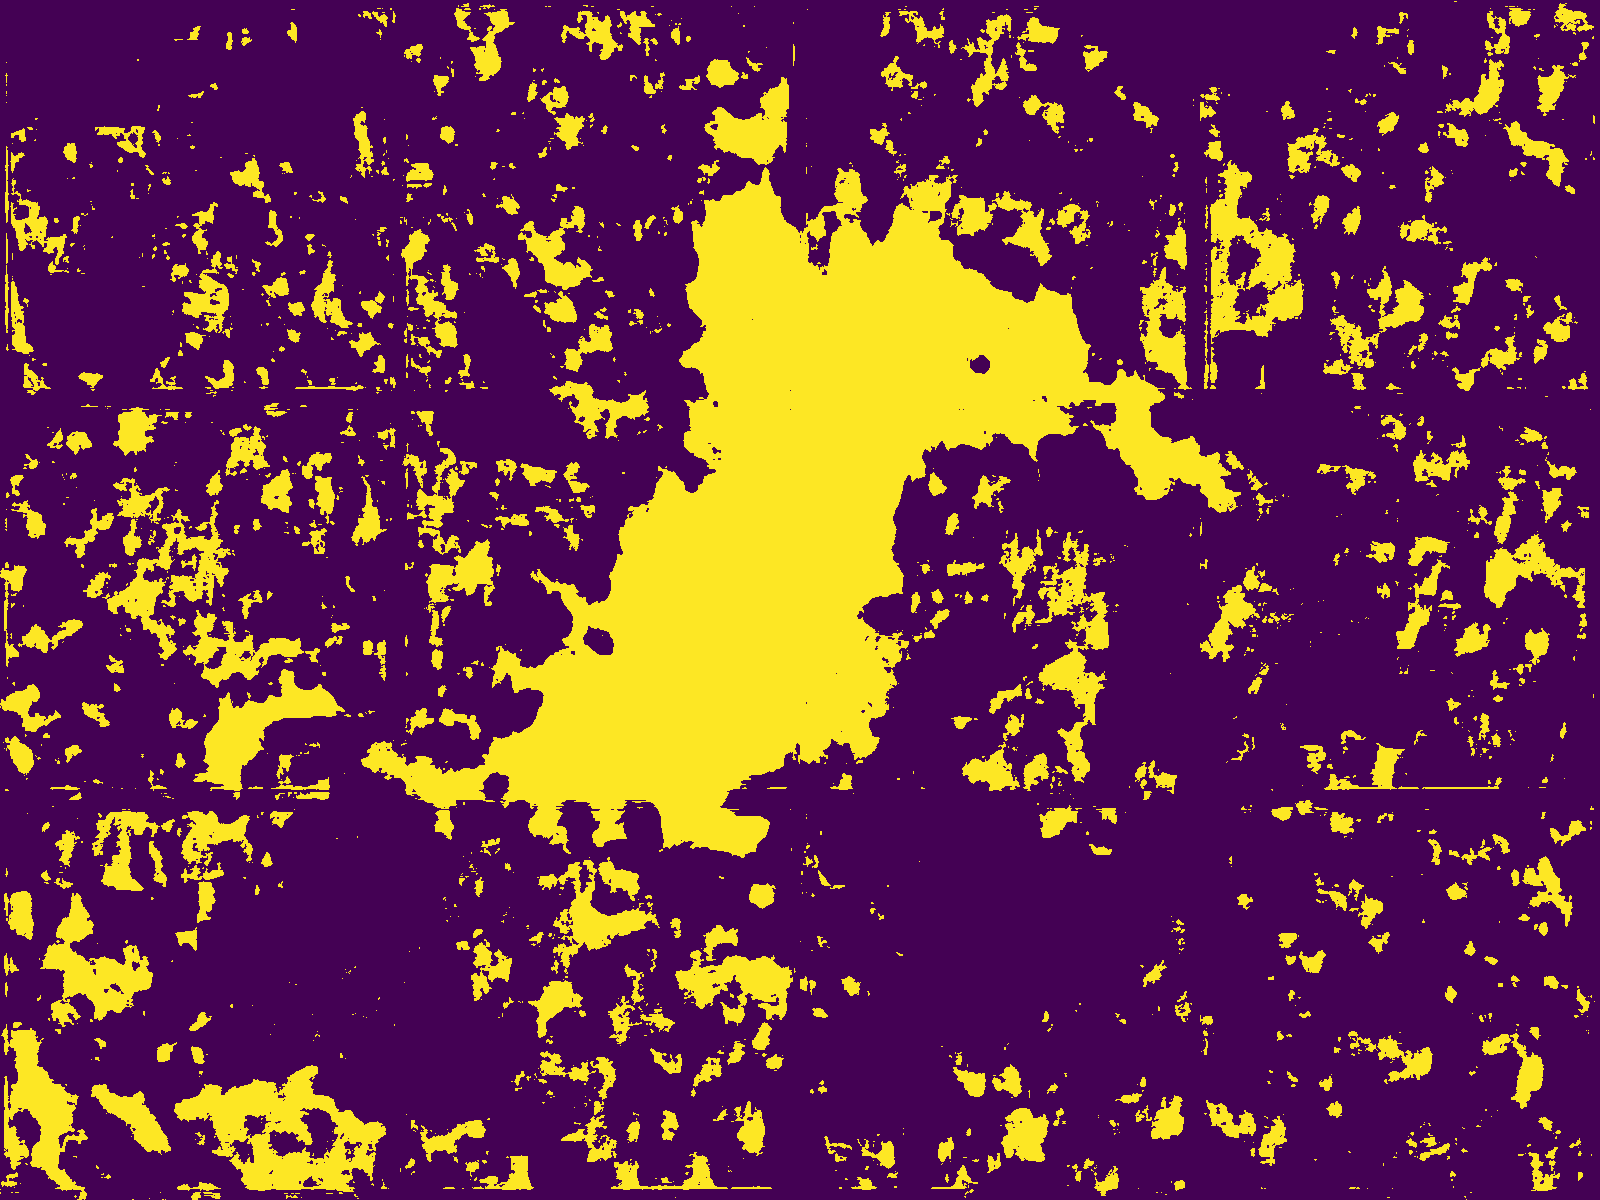
\includegraphics[width=0.32\linewidth]{figures/r20170802_185_7141.png}
}
\subfloat[258.6828 $km^2$]{
	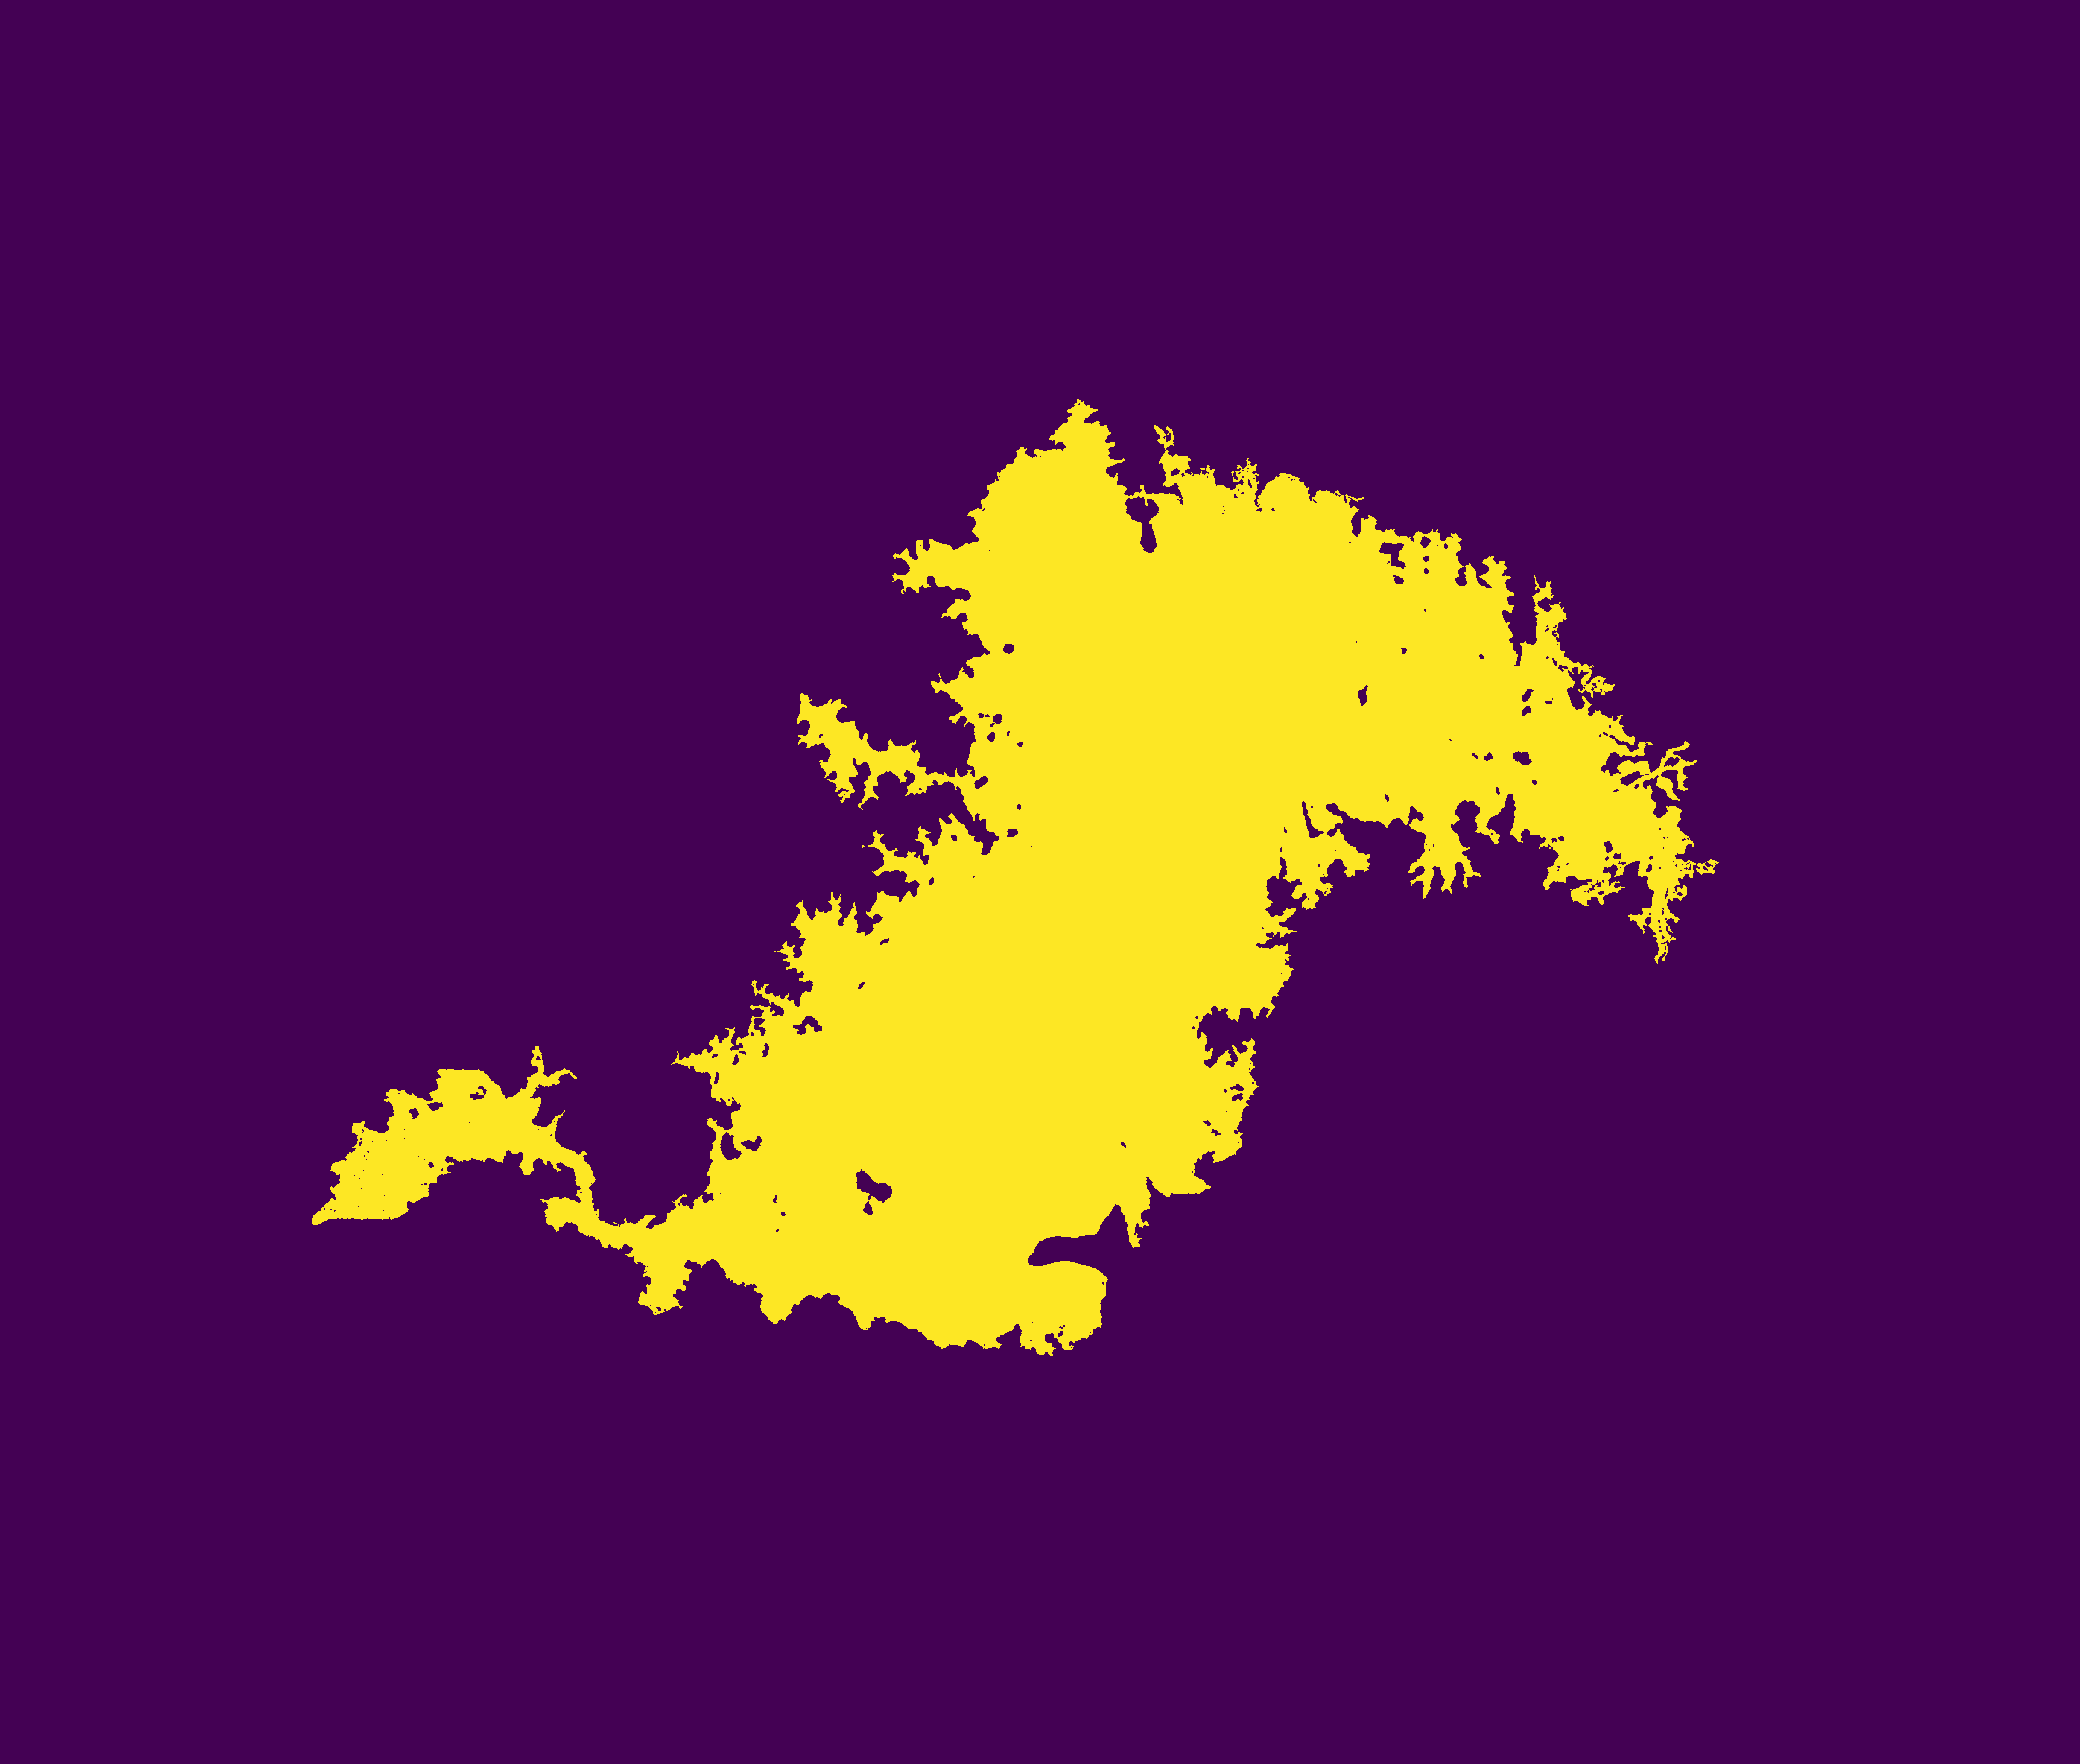
\includegraphics[width=0.32\linewidth]{figures/20170730_258_6828.png}
} 

\centering
\caption{
	\textbf{(a, b)} Landsat 8, Aug 2nd, 2017.
	\textbf{(c)} Sentinel-1, Jul 30th, 2017.}
\end{figure}

\subsection{Experiments on time-series data}

\subsubsection{Easiest case: Simple cloud shape}

\begin{figure}[h!]
	\centering
	\subfloat[]{
		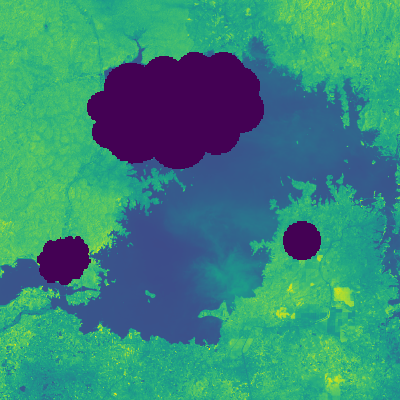
\includegraphics[width=0.24\linewidth]{figures/cont5_masked.png}
	}
	\subfloat[]{
		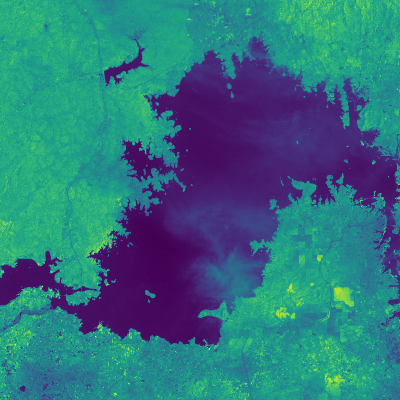
\includegraphics[width=0.24\linewidth]{figures/cont5_gt.png}
	}
	\subfloat[]{
		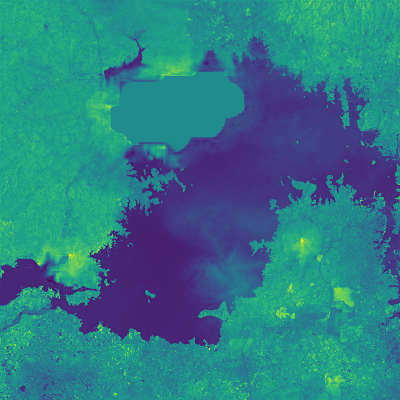
\includegraphics[width=0.24\linewidth]{figures/rcnn_simple.png}
	}
	\subfloat[]{
		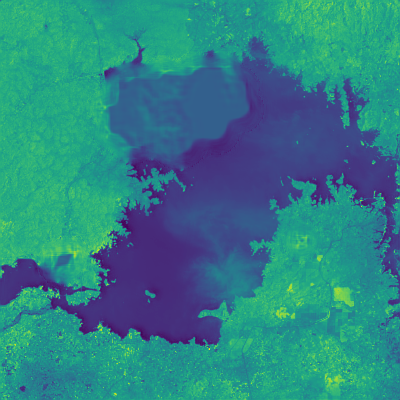
\includegraphics[width=0.24\linewidth]{figures/timecnn_simple.png}
	}  
	\centering
	\caption{Some clouds with simple shape}
\end{figure}

The result shows that for small regions, both methods could work well, but for a large missing region, it's not easy to get information from time-series images for recovery. Despite higher result in $PSNR$ metric, the recovered region by time-series images look worse than the single image as reference.

\subsubsection{Average case: Multi-simple cloud shape}

\begin{figure}[h!]
	\centering
	\subfloat[]{
		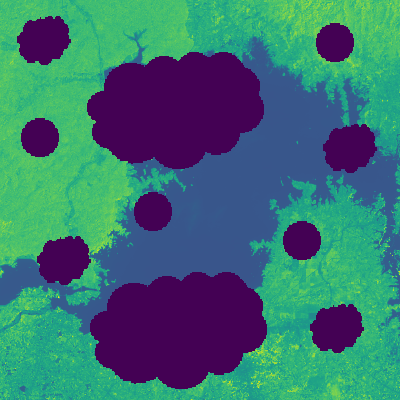
\includegraphics[width=0.24\linewidth]{figures/med_1.png}
	}
	\subfloat[]{
		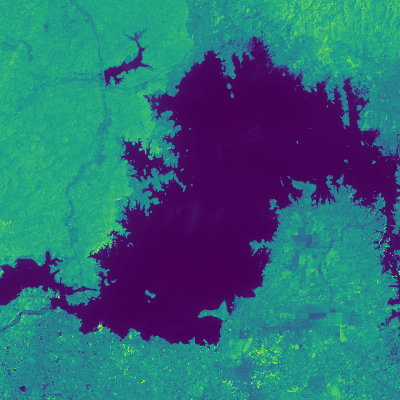
\includegraphics[width=0.24\linewidth]{figures/med_2.png}
	}
	\subfloat[]{
		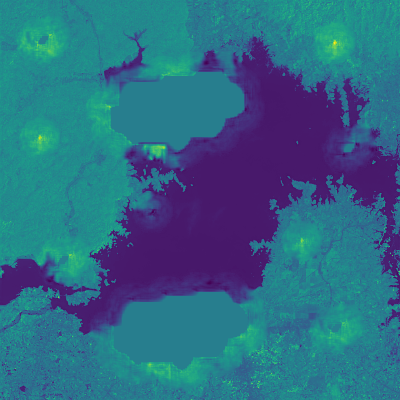
\includegraphics[width=0.24\linewidth]{figures/rcnn_med.png}
	}
	\subfloat[]{
		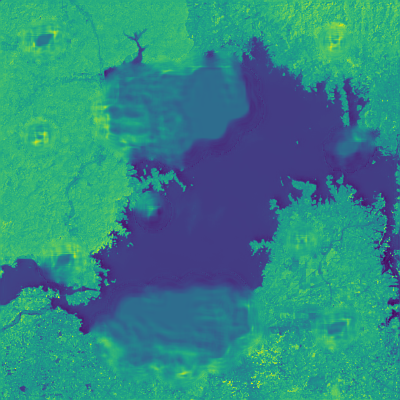
\includegraphics[width=0.24\linewidth]{figures/timecnn_med.png}
	}  
	\centering
	\caption{The result many clouds, in simple shape}
\end{figure}

\subsubsection{Hardest case: Real cloud}

\begin{figure}[h!]
	\centering
	\subfloat[]{
		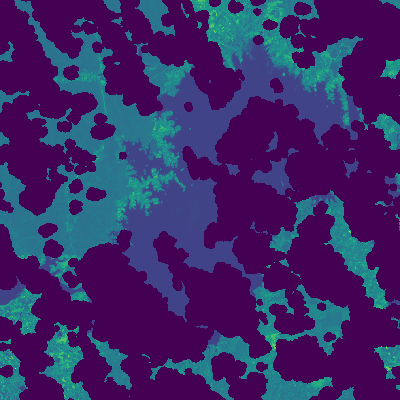
\includegraphics[width=0.24\linewidth]{figures/complext_1.png}
	}
	\subfloat[]{
		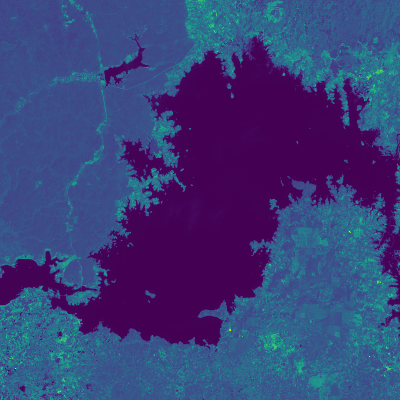
\includegraphics[width=0.24\linewidth]{figures/complext_2.png}
	}
	\subfloat[]{
		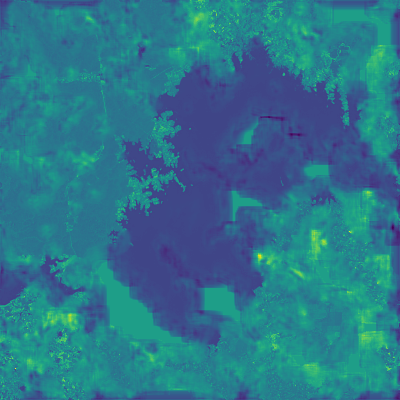
\includegraphics[width=0.24\linewidth]{figures/rcnn_complex.png}
	}
	\subfloat[]{
		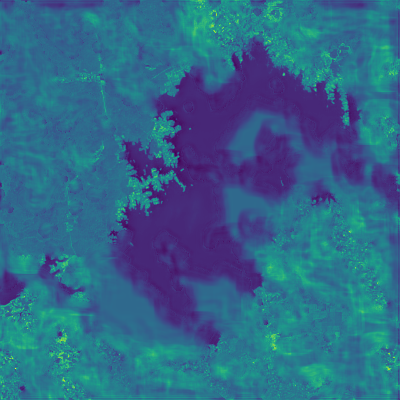
\includegraphics[width=0.24\linewidth]{figures/timecnn_complex.png}
	}  
	\centering
	\caption{The result on the most complex situation: Real cloud}
\end{figure}

\section{Conclusions}

For optimizing existing method: Scale image to range of $0..1$ slightly get better result than $0..255$. For range of $0..1$, $PSNR$ can be calculated faster as following, because $MAX_I = 1$, so $log_{10}(MAX_I) \textrm{ = } 0$ :

\begin{equation}
\centering
PSNR \textrm{ = } 20 * log_{10}(MAX_I) - 10 * log_{10}(MSE) \textrm{ = } -10 * log_{10}(MSE)
\end{equation}

Seemed to be more complex than original method, the modified model gives better result all over cases. Beside adding more one input to model, we've changed kernel filter of some layers. For some experiments, we found that larger kernel filter size gives better result, but adding more Convolutional layers doesn't. This looks like what mentioned in \textit{Image Super-Resolution Using Deep Convolutional Networks}, Chao et al.

Although the result of reconstruction is quite good when compare to existing method, when taking experiments on real images, it is not as good as expected. It might be quite good if only use it for a look. However, the model could be improved by not resizing the image to $400x400$ size. We could split it to tiles of $400x400$. It is not only keeping the original size, but also keeping details of original images, which is very good for training model.

The result of experiments on time-series images are not as good as expected. Firstly, the input as references for recovery part in network is only one (for a methods in \textbf{Chapter 3.2}, it is two). The second is, the sub-network for prediction is too simple. Itself is a very difficult problem. It is quite similar to a \textit{Moving MNIST problems}, for visualization, see at \href{http://www.cs.toronto.edu/~nitish/unsupervised_video/}{Department of Computer Science, Toronto University}. Some of papers has mentioned about it, for example, \textbf{Convolutional LSTM Network: A Machine Learning Approach for Precipitation Nowcasting}, Xingjian et al. So that, this sub-network have to be considered more complex. 
\chapter{Predict Water Body from Low-Resolution Satellite Images}
\label{chap-4-predict-water-body}
\begin{ChapAbstract}
In this chapter, ...
\end{ChapAbstract}

\section{Related Work}

\section{Model}

\section{Optimization}

\section{Experiments}

\section{Conclusions}


\chapter{Predict Water Body from Time-series High-Resolution Radar Satellite Images}
\label{chap-5-predict-from-sar-image}
\begin{ChapAbstract}
In this chapter, we would like to apply machine learning approach, especially deep learning, to predict the water body in the next future. We apply an extension on Long Short-Term Memory (LSTM), Conv-LSTM, to tackle problem. Conv-LSTM layer is not only take advantage from previous state-of-the-art approach in this kind of problems, Fully-Connected LSTM, but also very suitable to spatial-temporal data due to inherent convolutional structure. Because of the common things between water body and rainfall intensity in spatial and temporal information, we apply model from precipitation nowcasting problem to our prediction problem, modify about ways to train model, then Tri An Reservor is one more time selected to take experiment on. 

\end{ChapAbstract}

\section{Related Work}

% Time-series data prediction: Video / Precipitation Nowcasting.

Prediction (a.k.a. sequence prediction) is one of interesting fields in machine learning, in which the input (sequence data) contains an order on the observations and this order must be preserved while training model and making prediction.

\begin{figure}[h!]
	\centering
	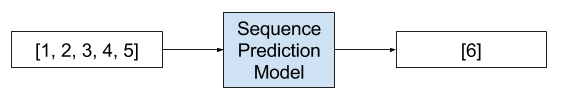
\includegraphics[width=0.7\textwidth]{figures/Example-of-a-Sequence-Prediction-Problem.png}
	\caption{Example of simple sequence prediction}
	\label{fig:exampleSimpleSequencePrediction}
\end{figure}

There are some example of sequence prediction problems, including:


\begin{enumerate}
	\item \textbf{Stock Market Prediction}\cite{Pagolu2016,Liu2018}. Given sequence of stock value as input, predict the expected next stock value. 
	
	\item \textbf{Product Recommendation}\cite{Wang2018,Cao2019}. Given sequence of recent purchased goods of a customer, predict the thing that the customer might "add to cart" next, and then make recommendation. 
	
	\item \textbf{Weather Forecasting}\cite{Quan2000,Wang2017}. Given sequence of weather observation over a period of time, predict the expected weather in next point of time.
	
\end{enumerate}

% Related to water body from satellite images, figure out why it related and its expansion: periodical information

One of important fields of weather forecasting is Nowcasting Precipitation\cite{Sun2013}. The goal of this task is about giving precise prediction of rainfall intensity in a region, over a short period of time. Recent advances in deep learning, Recurrent Neural Networks (RNNs), especially Long Short-Term Memories (LSTMs) models\cite{Graves2013GeneratingSW,Hochreiter1997,Cho2014,Donahue2017} provides good results on this kind of problem. In this thesis, we would like to predict the next water body shape (related to its area), from its time-series data. The common things between nowcasting precipitation and this problem is they both have spatial, spectral and temporal information inside data. We would like to apply model containing Conv-LSTM-2D layer\cite{Shi2015ConvolutionalLN}, to solve our proposed problem. Conv-LSTM-2D layer is recently used in computer vision, especially spatial-temporal problems. In this problem, we would like to extract the spatial feature as well as the correlation in the time. The fully-connected LSTMs can capture the temporal correlation but do not encode the spatial data. That's why they propose a model where the input to state and state to state transitions are convolutional. The model in \cite{Shi2015ConvolutionalLN} show better result on capturing spatial-temporal correlations than other state-of-the-art methods. So in this thesis, we will take this model as reference to provide solution for our problem, for Tri An reservoir.

\section{Dataset} 

In this chapter, Tri An reservoir is chosen for experiments. Because Radar Satellites Images is not affected by cloud cover like optical satellite in \ref{chap-3-recover-water-body}, so we only focus on prediction water body. The synthetic-aperture radar \footnote{https://en.wikipedia.org/wiki/Synthetic-aperture\_radar} monthly imagery provided from Sentinel-1 satellites \footnote{https://sentinel.esa.int/web/sentinel/missions/sentinel-1} are collected from \textit{November 25tr, 2015} to \textit{June 1st, 2019} for training and evaluating. 

Depending on coordinates of Tri An Reservoir, the original image has been cropped to size \textit{2560 px} x \textit{3840 px}, enough to show its water body.

\subsection{Water body segmentation on Sentinel-1 Image}

Sentinel-1 Satellite provides image with 10m spatial resolution. In this thesis, in order to segment out water body, we depend on VH or VV polarizations imagery and apply corresponding threshold:

\begin{equation}
\centering
VH \leq -21
\end{equation} 

\begin{equation}
\centering
VV \leq -17
\end{equation} 

Because in our cropped image that only contains Tri An Reservoir as the largest water body, so we only need to find out the most largest one, using Bread-First Search algorithm\footnote{https://en.wikipedia.org/wiki/Breadth-first\_search}. With this object, we easily to figure out the boundaries, with help of function \textit{find\_boundaries}, from Python library \textit{Scikit-Image}\footnote{https://scikit-image.org/}.

\section{Model}

The model has been implemented by Keras. Its structure is shown below:

\begin{figure}[h!]
	\centering
	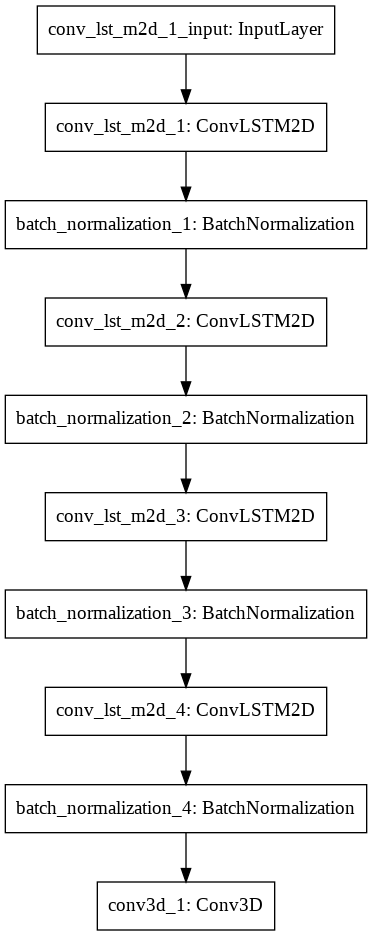
\includegraphics[width=0.5\textwidth]{figures/time_model.png}
	\caption{Prediction mode, based on Conv-LSTM-2D}
	\label{fig:timeModel}
\end{figure}

Model summary detail:

\begin{verbatim}
_________________________________________________________________
Layer (type)                 Output Shape               Param #   
=================================================================
conv_lst_m2d_1 (ConvLSTM2D)  (None, None, 128, 128, 64) 815616    
_________________________________________________________________
batch_normalization_1 (Batch (None, None, 128, 128, 64) 256       
_________________________________________________________________
conv_lst_m2d_2 (ConvLSTM2D)  (None, None, 128, 128, 32) 602240    
_________________________________________________________________
batch_normalization_2 (Batch (None, None, 128, 128, 32) 128       
_________________________________________________________________
conv_lst_m2d_3 (ConvLSTM2D)  (None, None, 128, 128, 32) 401536    
_________________________________________________________________
batch_normalization_3 (Batch (None, None, 128, 128, 32) 128       
_________________________________________________________________
conv_lst_m2d_4 (ConvLSTM2D)  (None, None, 128, 128, 32) 401536    
_________________________________________________________________
batch_normalization_4 (Batch (None, None, 128, 128, 32) 128       
_________________________________________________________________
conv3d_1 (Conv3D)            (None, None, 128, 128, 1)  33        
=================================================================
Total params: 2,221,601
Trainable params: 2,221,281
Non-trainable params: 320
_________________________________________________________________
\end{verbatim}

Specification:

\begin{itemize}
	\item \textit{Input and Output} Because we only focus on predicting water body, so after extracting water body from original image and finding out its boundaries, we randomize on boundaries 50 tiles with size of 128 x 128. There is 12 consecutive images, corresponding to 12 month in year. The output is a image of next month, which is same month of 1st image in input sequence but next year. 
	
	\item \textit{Conv3D} This type of layer helps to catch spatial and temporal invariances in the same manner as \textit{Conv2D} in an imagery case. This make the curse of dimensionality much less harmful. Because at the end of model, we need to have a prediction, so it's no longer to keep temporal information after this layer.
	
	\item \textit{Batch Normalization} Batch normalization reduces the amount by what the hidden unit values shift around (covariance shift). Morever, this layer allows each layer of a network to learn by itself a little bit more independently of other layers.
	
	\item \textit{Activation} The activation for Conv-LSTM-2D is $tanh$ function, for Conv3D is $sigmoid$ function.
	
	\item \textit{Dropout and Recurrent Dropout} In Recurrent Neural Networks, we have two definition about \textbf{Dropout} and \textbf{Recurrent Dropout}. \textbf{Dropout} describes fraction of the units to drop for the linear transformation of the inputs, while \textbf{Recurrent Dropout} show fraction of the units to drop for the linear transformation of the recurrent state (more detail at \cite{Gal2015}). In this model, with each Conv-LSTM-2D layer's configuration, $dropout$ is set at $0.4$, and and $recurrent\_dropout$ is $0.3$.
	
	\item \textit{Model compilation parameters} Like model compilation in \ref{chap-3-recover-water-body}, the loss function is still $mean_square_error$, optimizer is $adam$ and evaluation metric is $PSNR$(\ref{psnr_eq}). 
	
\end{itemize}

\section{Experiments}

\subsection{Prediction water body area}

% Show demo 12 input in 1 line

% Show table, contains result

% Plot predicted result, with groundtruth value

% Show 2-6/19 prediction, with result and boundaries.

\subsection{Anomaly sample}

% Plot anomaly in previous time

% Show image

% etc...



\section{Conclusions}


\chapter{Conclusions}
\label{chap-6-conclusions}
\begin{ChapAbstract}
In this chapter, ...
\end{ChapAbstract}




%%%%%%%%%%%%%%%%%%%%%%%%%%%%%%%%%%%%%%%%%%%%%%%%%%%%%%%
% The bibliography. Turn on page numbering.
%%%%%%%%%%%%%%%%%%%%%%%%%%%%%%%%%%%%%%%%%%%%%%%%%%%%%%%
\addtocontents{toc}{\protect\cftpagenumberson{chap}}
%%%% Soooo if IPS says there should be 5cm top margin
%%%% on the ``References'' heading page, uncomment the
%%%% line just before and after \bibliography. Repeat for
%%%% \bibliographyown if necessary
%% Increase spacing before chapter heading
\titlespacing*{\chapter}{0pt}{\dimexpr2.5cm-50pt}{\baselineskip}
\bibliography{refs}
% \bibliographystyle{plain}
% now change it back to normal
\titlespacing*{\chapter}{0pt}{-50pt}{\baselineskip}

%%%%%%%%%%%%%%%%%%%%%%%%%%%%%%%%%%%%%%%%%%%%%%%%%%%%%%%
% The appendices.
% If you don't have any, you may delete everything below,
% until and including % \include{app-paper}.
%%%%%%%%%%%%%%%%%%%%%%%%%%%%%%%%%%%%%%%%%%%%%%%%%%%%%%%
\appendix
\assignpagestyle{\chapter}{empty}
% * If IPS says they don't want any page numbering in the footer,
%   add \pagestyle{empty}
% * If they don't want any page numbering in the ToC either,
%   add \addtocontents{toc}{\protect\cftpagenumbersoff{chap}}
% * If they say they don't want Appendix A, B, C... to appear
%   in the ToC either, add
%     \addtocontents{toc}{\protect\setcounter{tocdepth}{-1}}
%     \addtocontents{toc}{\texbf{List of Publications}} % (to get it to appear)
% \include{app-paper}
\assignpagestyle{\chapter}{plain}

%%%%%%%%%%%%%%%%%%%%%%%%%%%%%%%%%%%%%%%%%%%%%%%%%%%%%%%
% The list of own publications.  If you don't have one, you may
% comment out the next 4 lines.
%%%%%%%%%%%%%%%%%%%%%%%%%%%%%%%%%%%%%%%%%%%%%%%%%%%%%%%
% Uncomment/comment this line if you need the List of Publications to be bold/not bold in the ToC.
\addtocontents{toc}{\protect\renewcommand\protect\cftchapfont{\protect\bfseries}}
\nociteown{3dor.20181052}
\bibliographyown{mybib}

\end{document}
